\section{Results}


\subsection{Principal components analysis}
\label{sec:PCAresults}
One of the papers that served as initial inspiration for this research project was \cite*{Clark2015}. \cite{Clark2015} used principal component analysis on the gravitational-wave spectra of the  signals for various EOS and mass values. Principal component analysis (PCA) uses a decomposition process to order principal components from most significant to least significant, specific details are shown in section~\ref{sec:PCA}.\color{black}\ Each principal component corresponds to one axis in PCA space, and the coefficients created from the decomposition of an individual waveform are represented by a single point in the PCA space. PCA decomposition does not give any information on what each of the principal components represent, but it can be useful for categorisation and finding relationships between different signals. We performed PCA decomposition on both  scaled (section \ref{sec:PCAScaled}) and  unscaled (section \ref{sec:PCAUnscaled}) frequency waveforms. 
% ClarkReplication.ipynb

% Cumulative explained variances were not reproduced as per Clark, convergence based on the number of principal components was much slower. 

\subsubsection{Scaled Frequency}
\label{sec:PCAScaled}
Before performing PCA decomposition on their waveforms, \cite{Clark2015} implemented frequency scaling on their data. The new frequency values were calculated as  shown in equation~\ref{eq:fscaling}:
\begin{equation}
	F_j^{'}=F_j\left(\dfrac{f_{\text{peak}}}{f_{\text{peak-}j}}\right),
	\label{eq:fscaling}
\end{equation} 
where $f_{\text{peak-}j}$ is the frequency corresponding to the peak amplitude of the FFT for waveform $j$. The peak frequency value, $f_{\text{peak}}$ is a free value that can be chosen. We used the same frequency scaling as \cite{Clark2015} to generate PCA decomposition on our waveforms with three principal components. An important consideration was that the frequency values for one waveform to the next no longer matched after this transformation. Furthermore, it was necessary to have a common frequency value for each of the FFT waveforms to enable PCA analysis on the data. Because of this, the complex FFT amplitude, $H_j$, was interpolated onto a fixed set of frequency values which were set to be the same for all waveforms. Note also that it was necessary to reverse this transform before performing an inverse FFT to generate time series data.\par The frequency range was restricted from 600 to 8000Hz, which is the frequency range of interest for the post-merger signals. The PCA decomposition was performed on both the amplitude and phase of the Fourier spectrum. Figure~\ref{fig:PCAScaled3Damp} shows the result of this decomposition for the amplitude of the Fourier spectra. 
\begin{figure}[H]
	\centering
	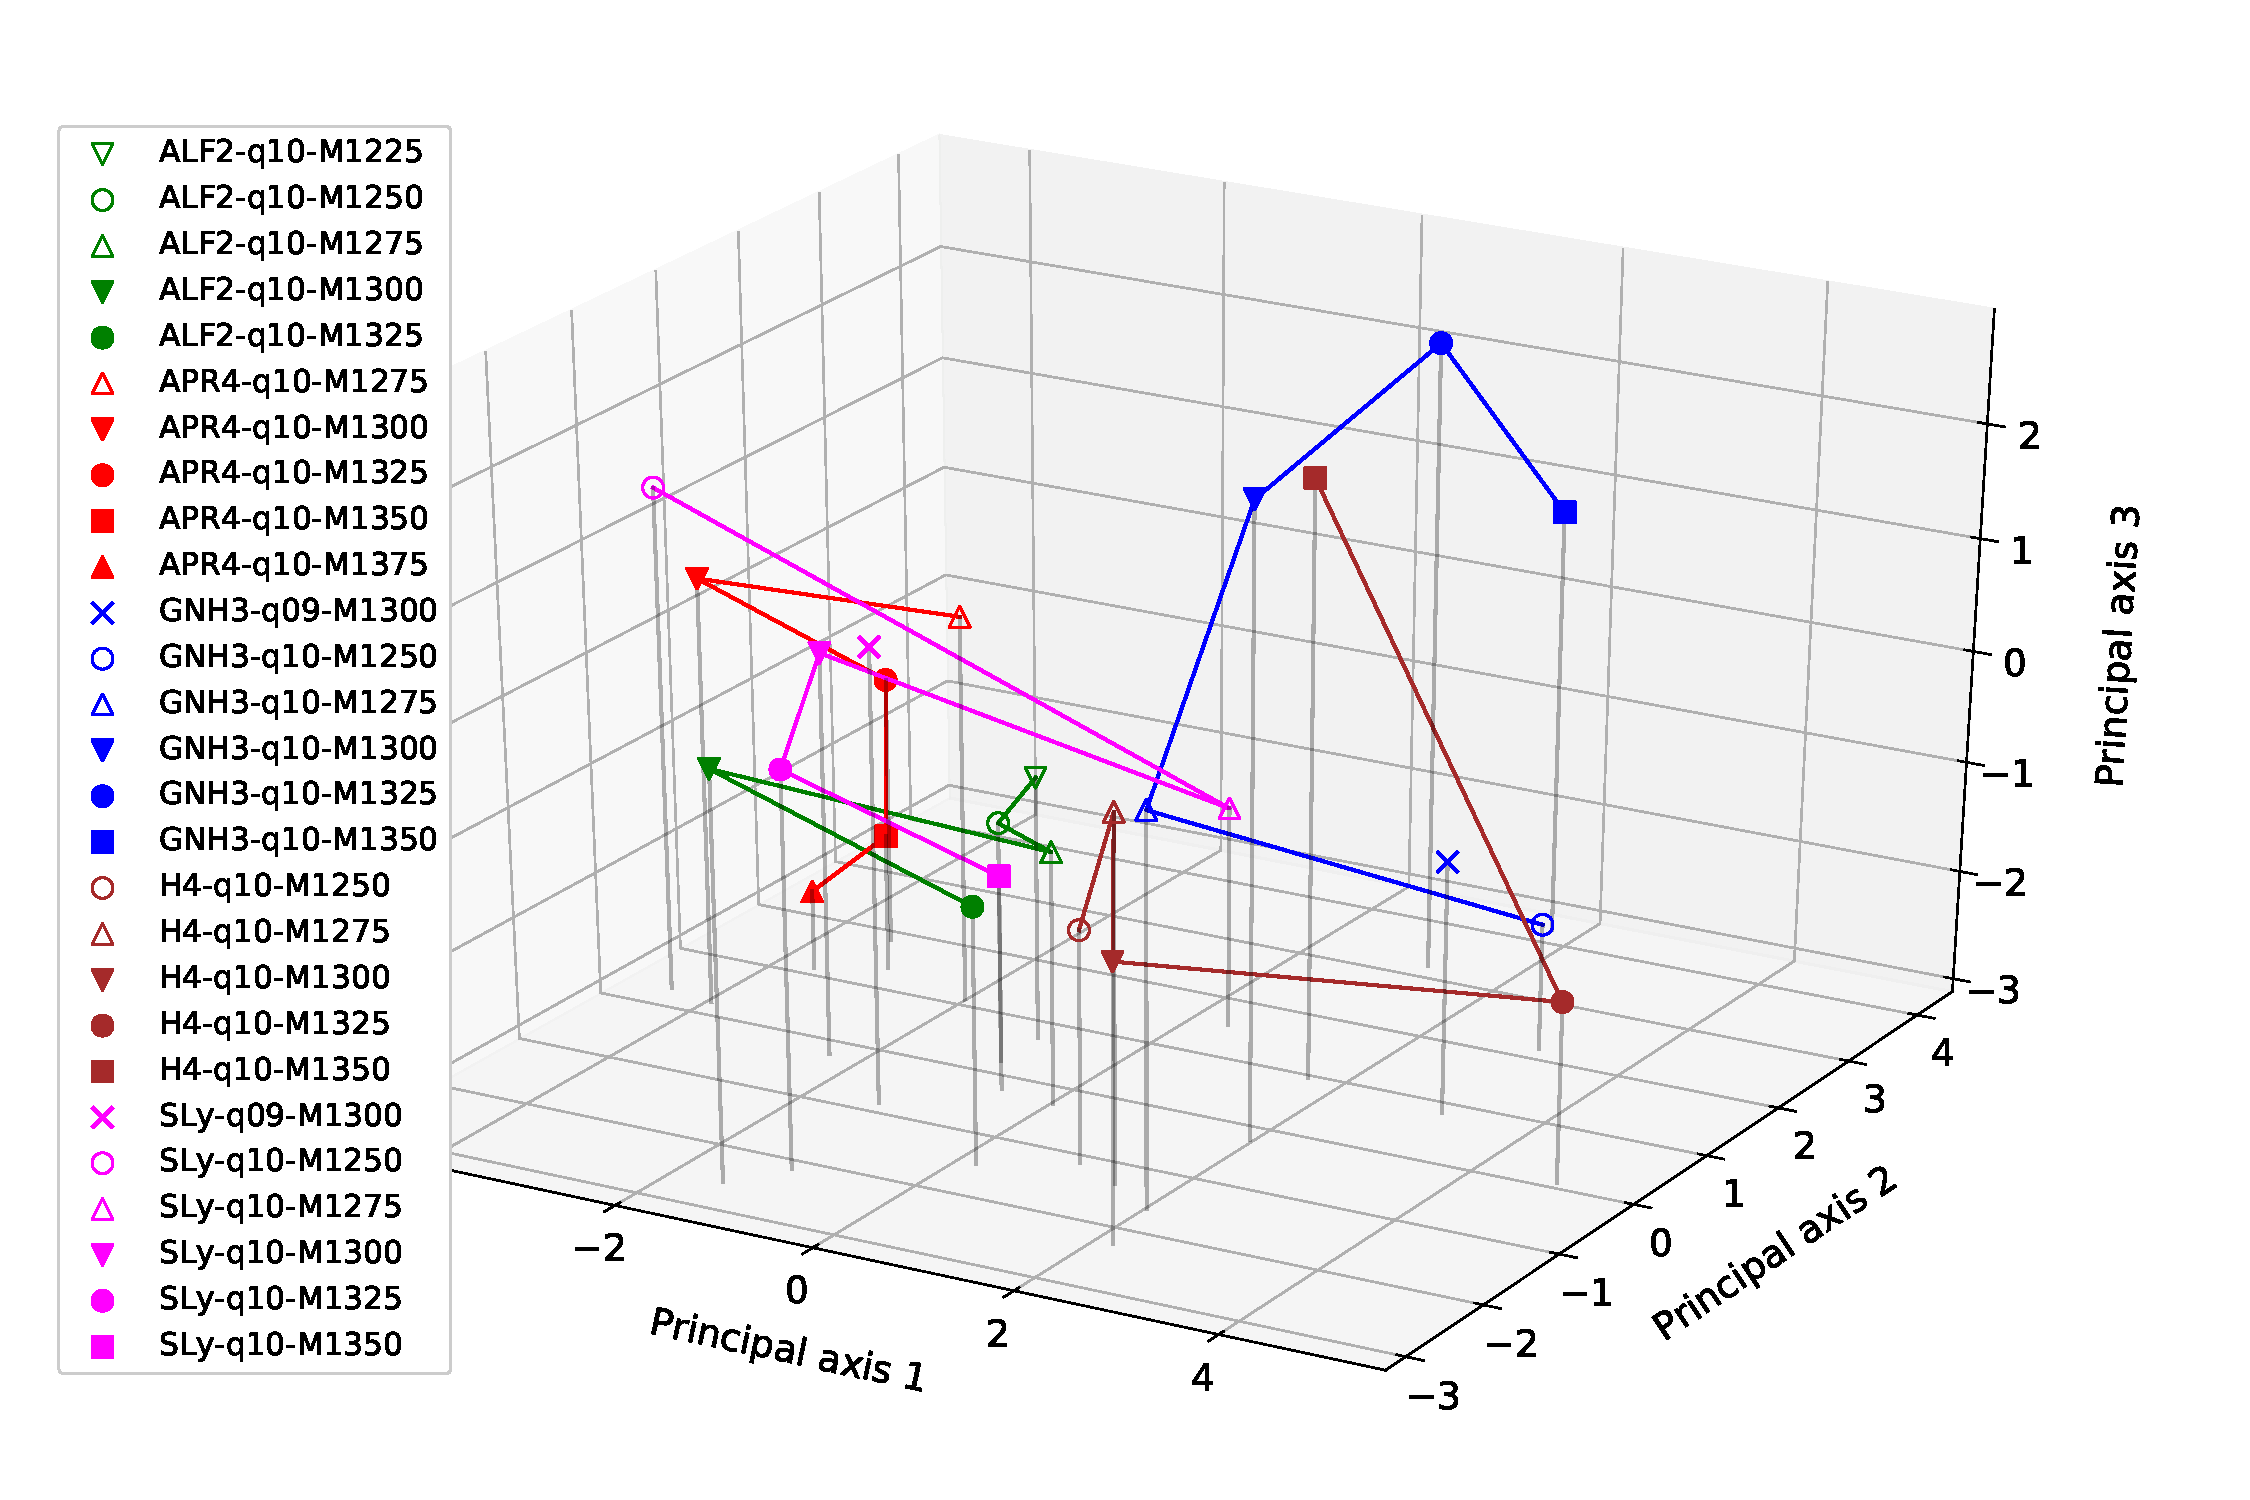
\includegraphics[width=15cm]{./img/PCAScaled3Damp.pdf} 
	\caption[\protect\input{./img/PCAScaled3DampShort.txt}]{\protect\input{./img/PCAScaled3Damp.txt}}
	\label{fig:PCAScaled3Damp}
\end{figure}
Each EOS is shown in a different colour, corresponding to the same colours used in figures~\ref{fig:hEOS}~and~\ref{fig:fEOS}. For equal mass systems ($q=1.0$) a line was drawn to connect adjacent mass values for the same EOS. This was to aid in determining whether any pattern or correlation could be visually seen corresponding to increasing mass, but the locus through the PCA space appears disjointed. The waveforms are designated as follows: EEEE-QQQ-MYXXX, where: 1) EEEE is the EOS used, 2) QQQ is the mass ratio, either 1.0 (q10) or 0.92593 (q09), 3) MYXXX is the mean mass value of both neutron stars with a mass of Y.XXX, so M1350 refers to a system with mean mass of 1.350M$_\odot$. Vertical grey lines were projected downward to the X,Y plane of the principal axes 1 and 2, to aid visual placement of the markers in the three dimensional space. Projecting this information down to the XY plane aids the interpretation of this plot  and is shown in figure~\ref{fig:PCAScaled2Damp}.
\begin{figure}[H]
	\centering
	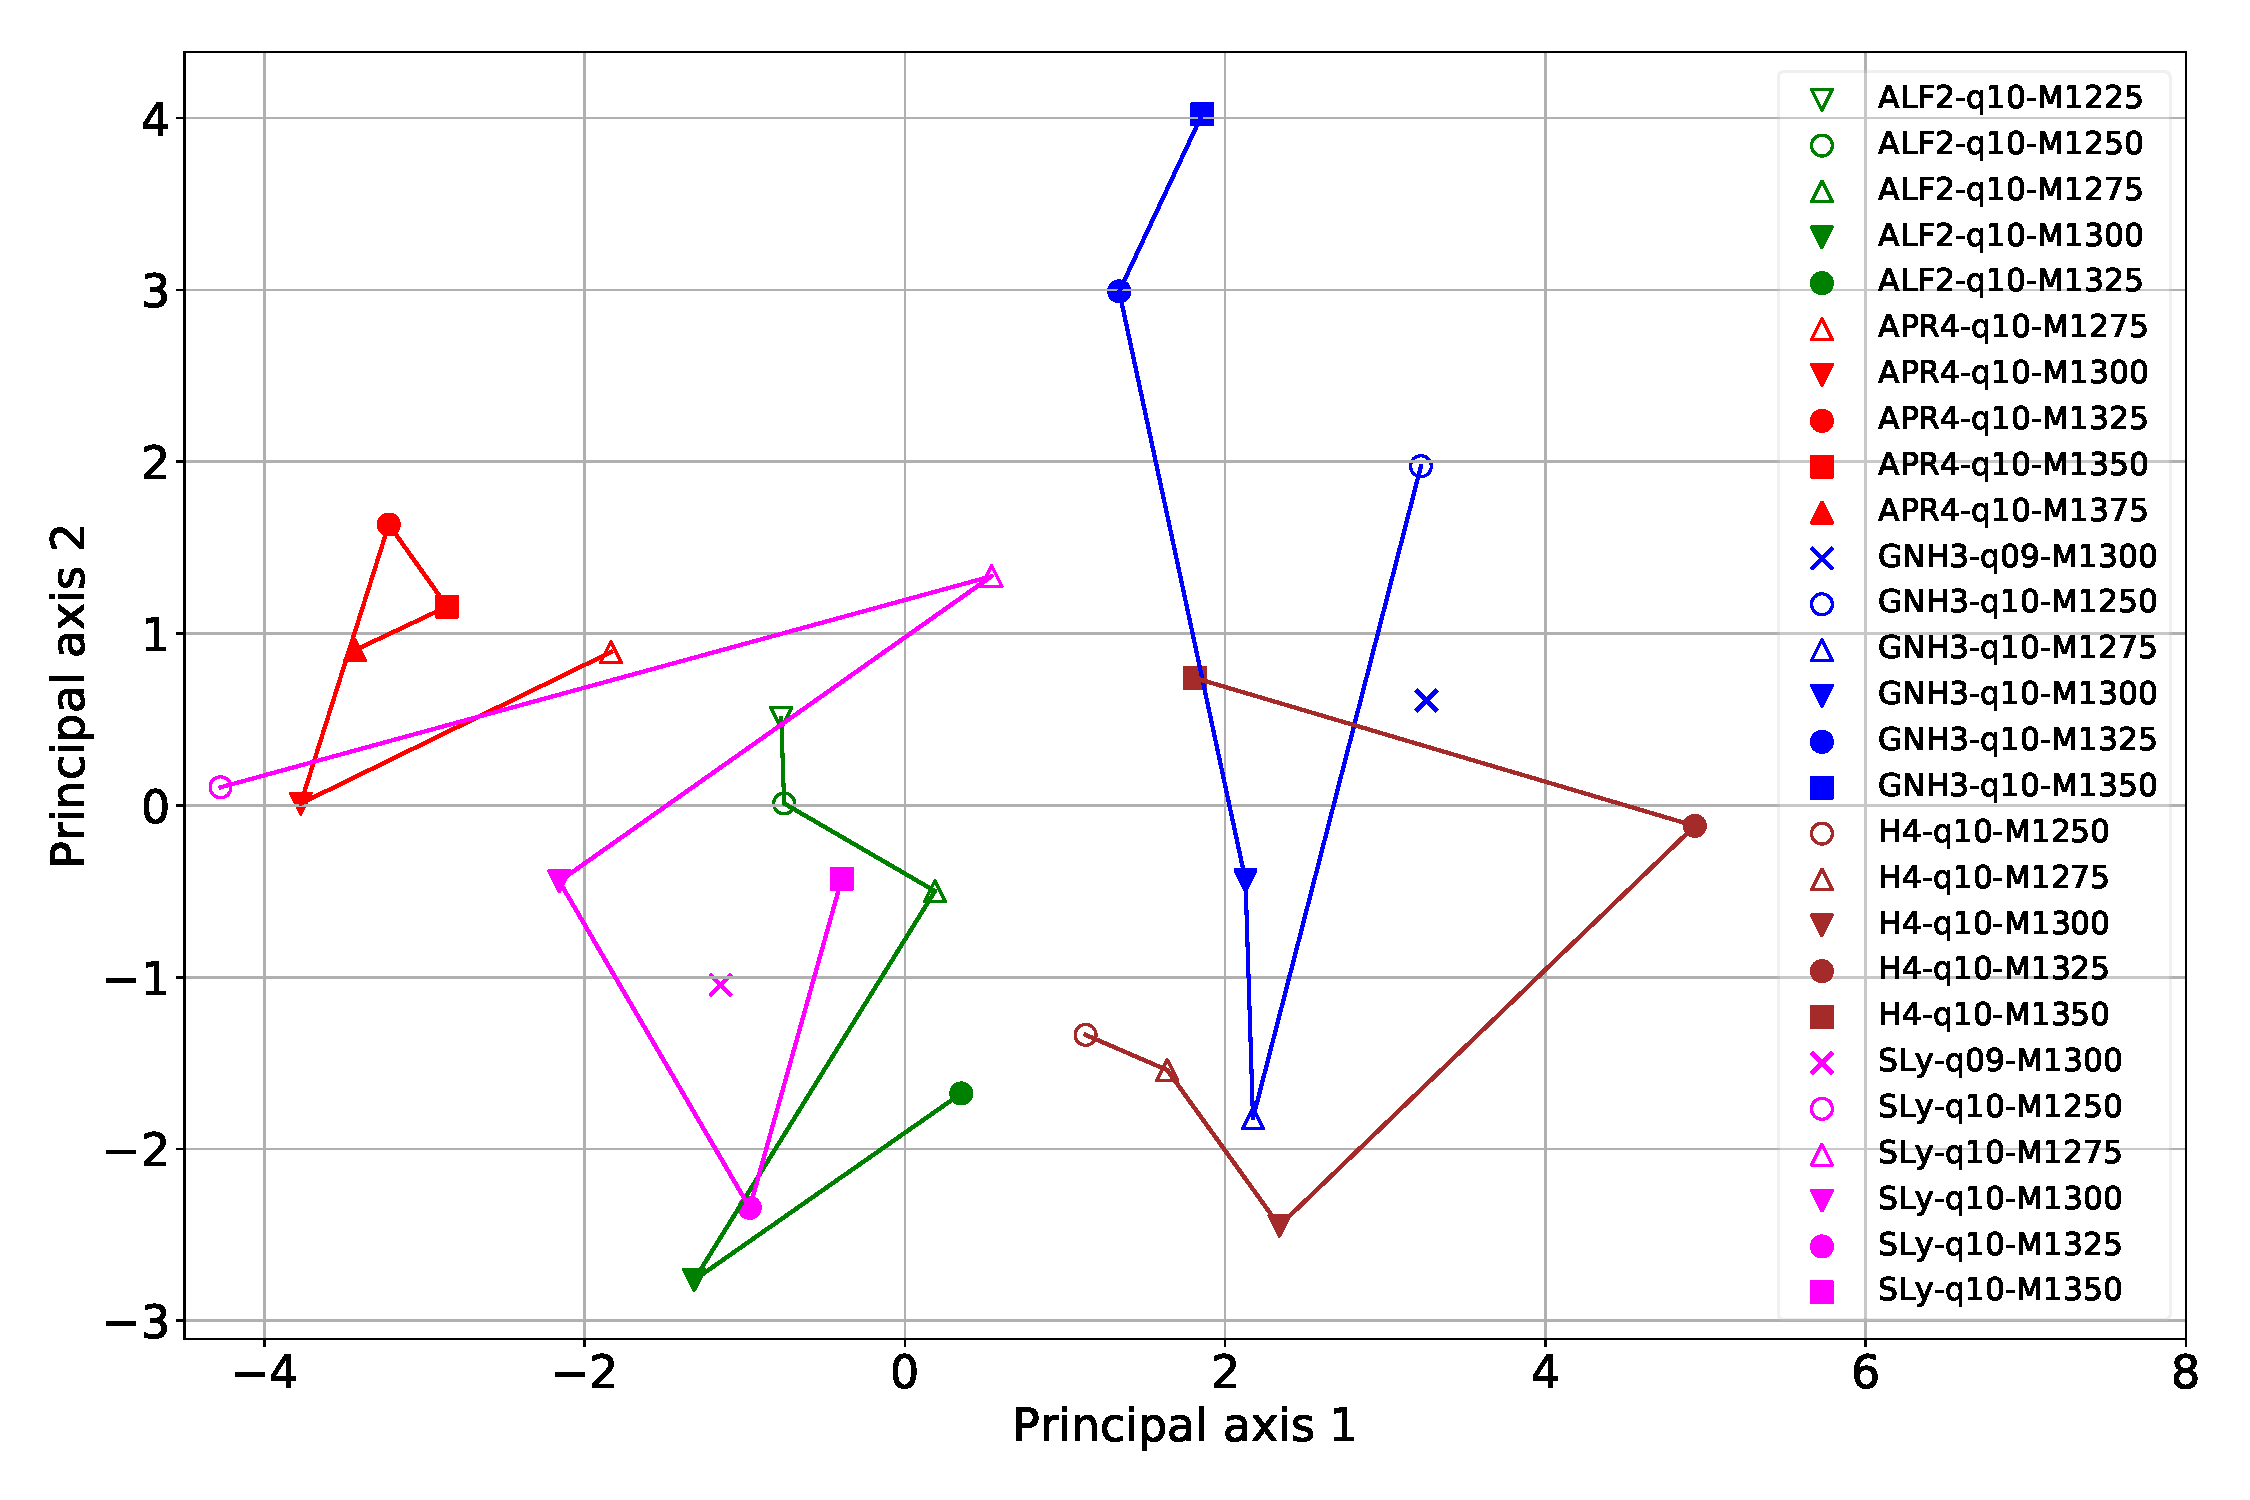
\includegraphics[width=15cm]{./img/PCAScaled2Damp.pdf} 
	\caption[\protect\input{./img/PCAScaled2DampShort.txt}]{\protect\input{./img/PCAScaled2Damp.txt}}
	\label{fig:PCAScaled2Damp}
\end{figure}
The H4 and the GNH3 EOS occupy roughly the same part of the PCA space, and the other three EOSs, ALF2, APR4 and SLy, occupy another distinct part of PCA space. However, when comparing  with tables~\ref{tbl:Waveforms1Table}~and~\ref{tbl:Waveforms2Table}, there is no clear parameter that allows for this distinction between these two classes of EOS. Another important consideration is that the locus through the PCA space is still quite disjointed, and difficult to find correlations by eye, but this may be such a situation where machine learning can aid in the determination of any correlations. \par 
Figure~\ref{fig:PCAScaled3Dphase} shows the corresponding phase response for the frequency scaled waveforms in three component PCA space.
\begin{figure}[H]
	\centering
	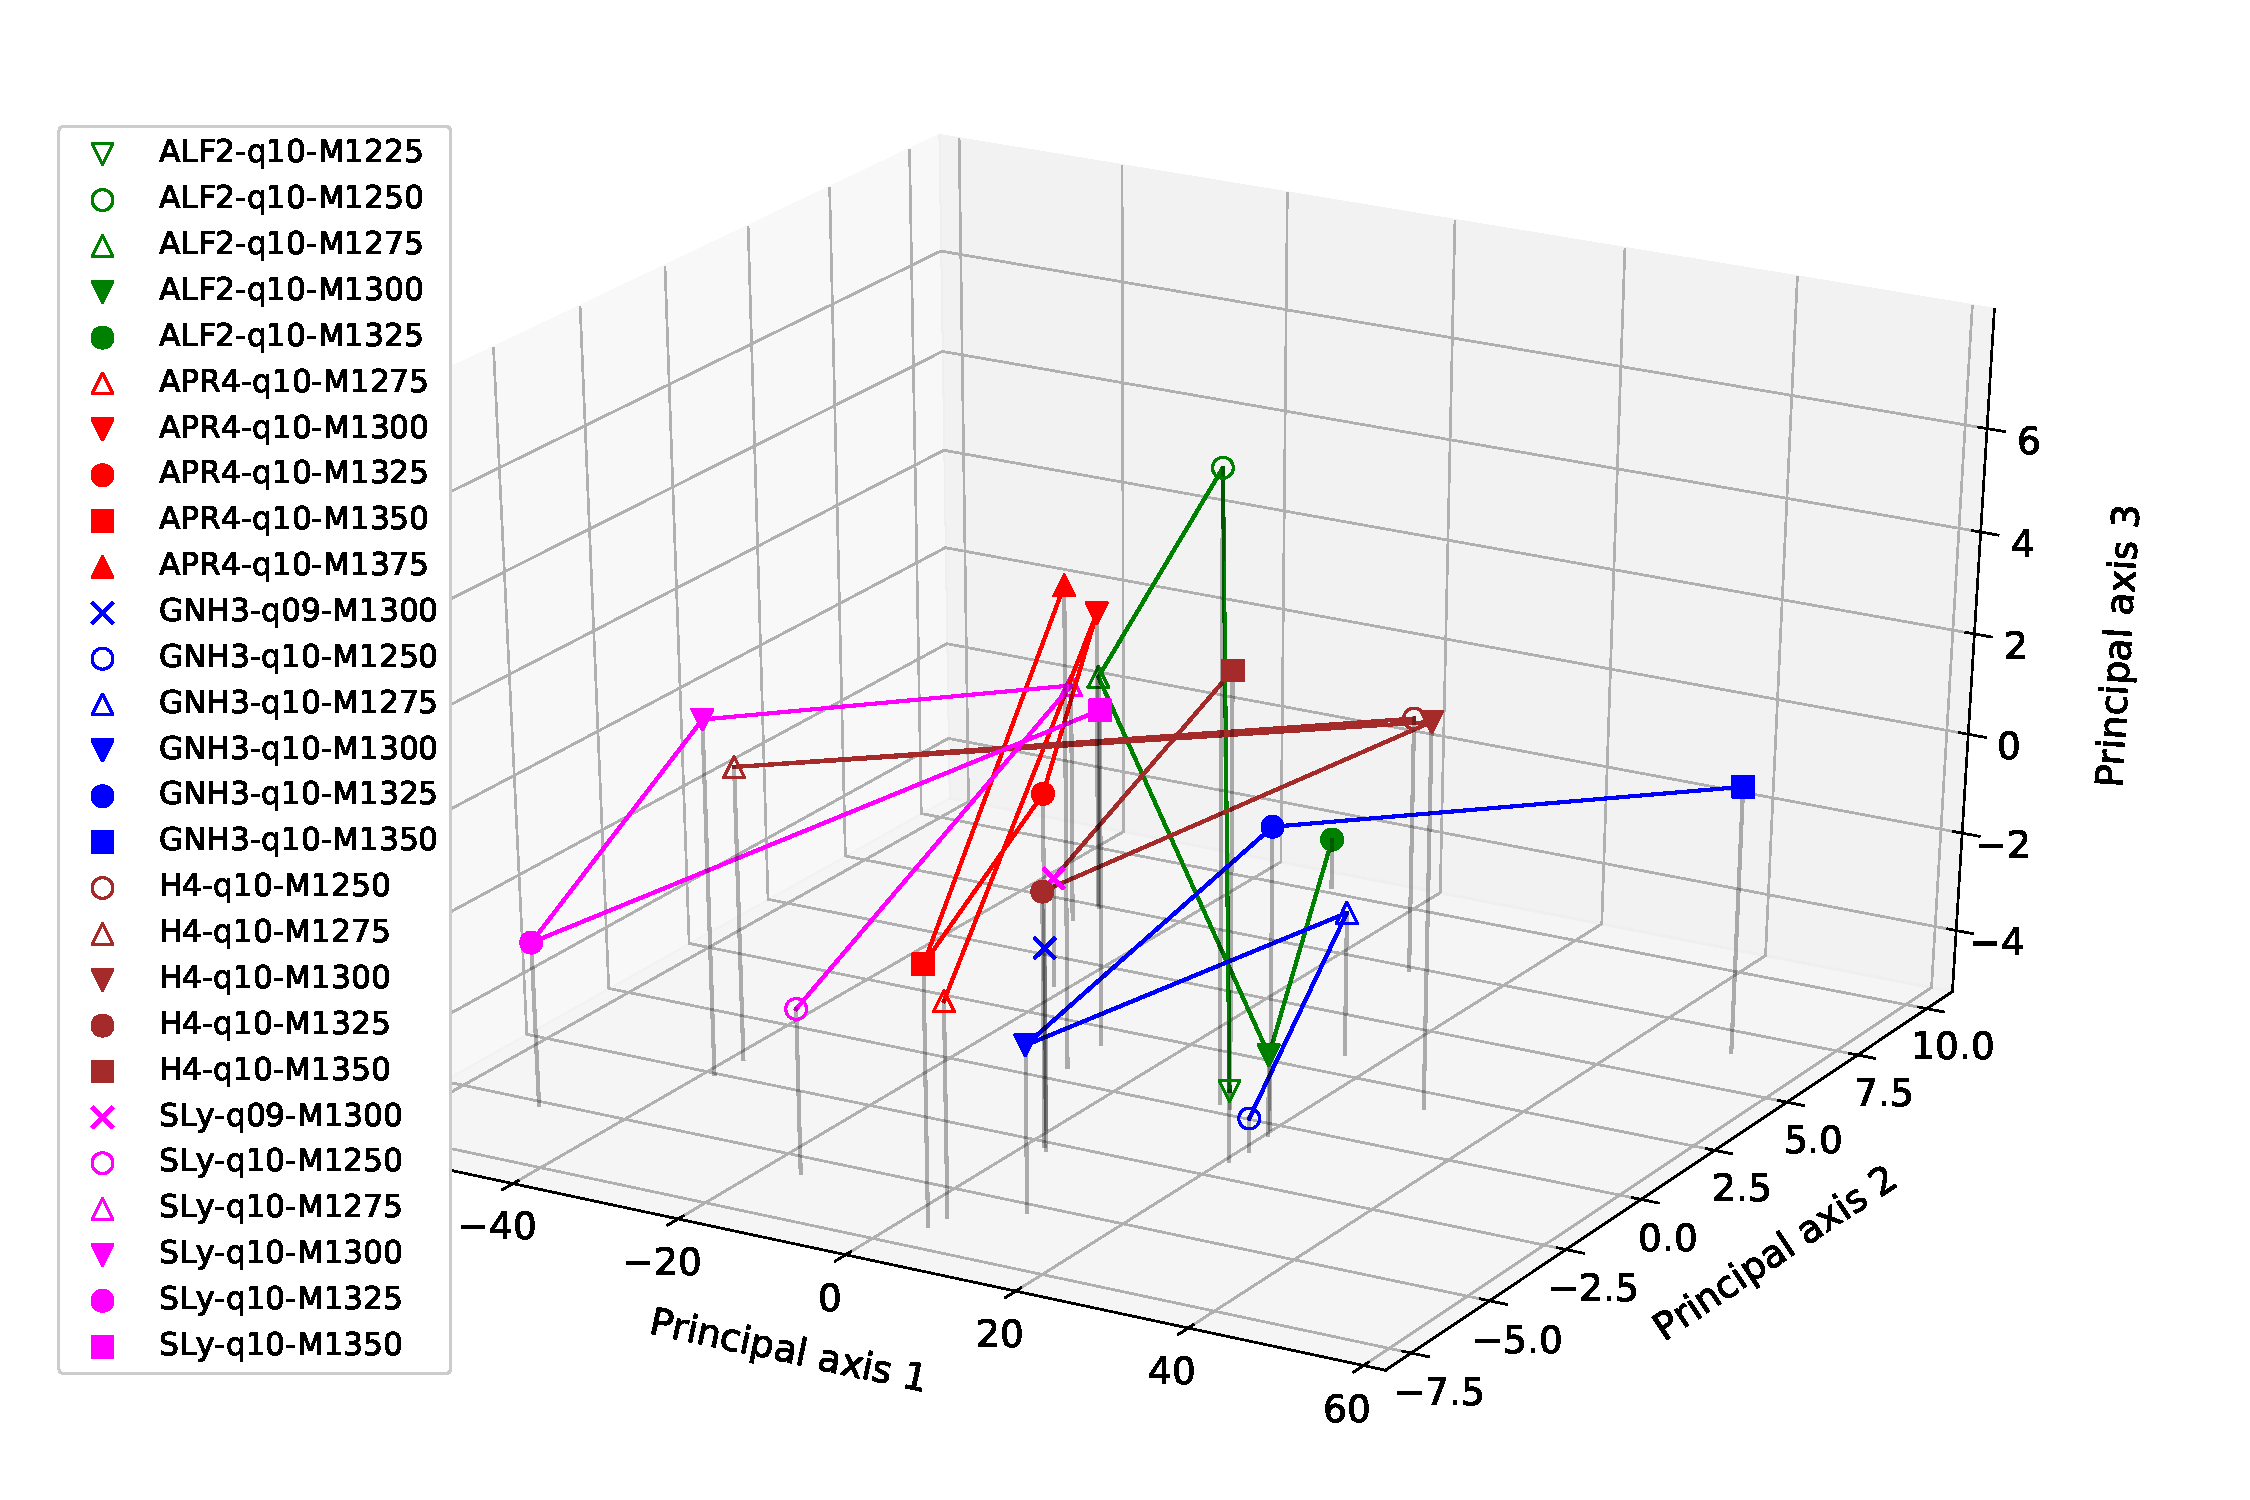
\includegraphics[width=15cm]{./img/PCAScaled3Dphase.pdf} 
	\caption[\protect\input{./img/PCAScaled3DphaseShort.txt}]{\protect\input{./img/PCAScaled3Dphase.txt}}
	\label{fig:PCAScaled3Dphase}
\end{figure}
The distinction between different EOS in PCA phase space is even more difficult, the different points in phase space appear to exhibit significant overlap. Figure~\ref{fig:PCAScaled2Dphase} shows the projection of figure~\ref{fig:PCAScaled3Dphase} down to the XY plane to aid in the analysis of this data.
\begin{figure}[H]
	\centering
	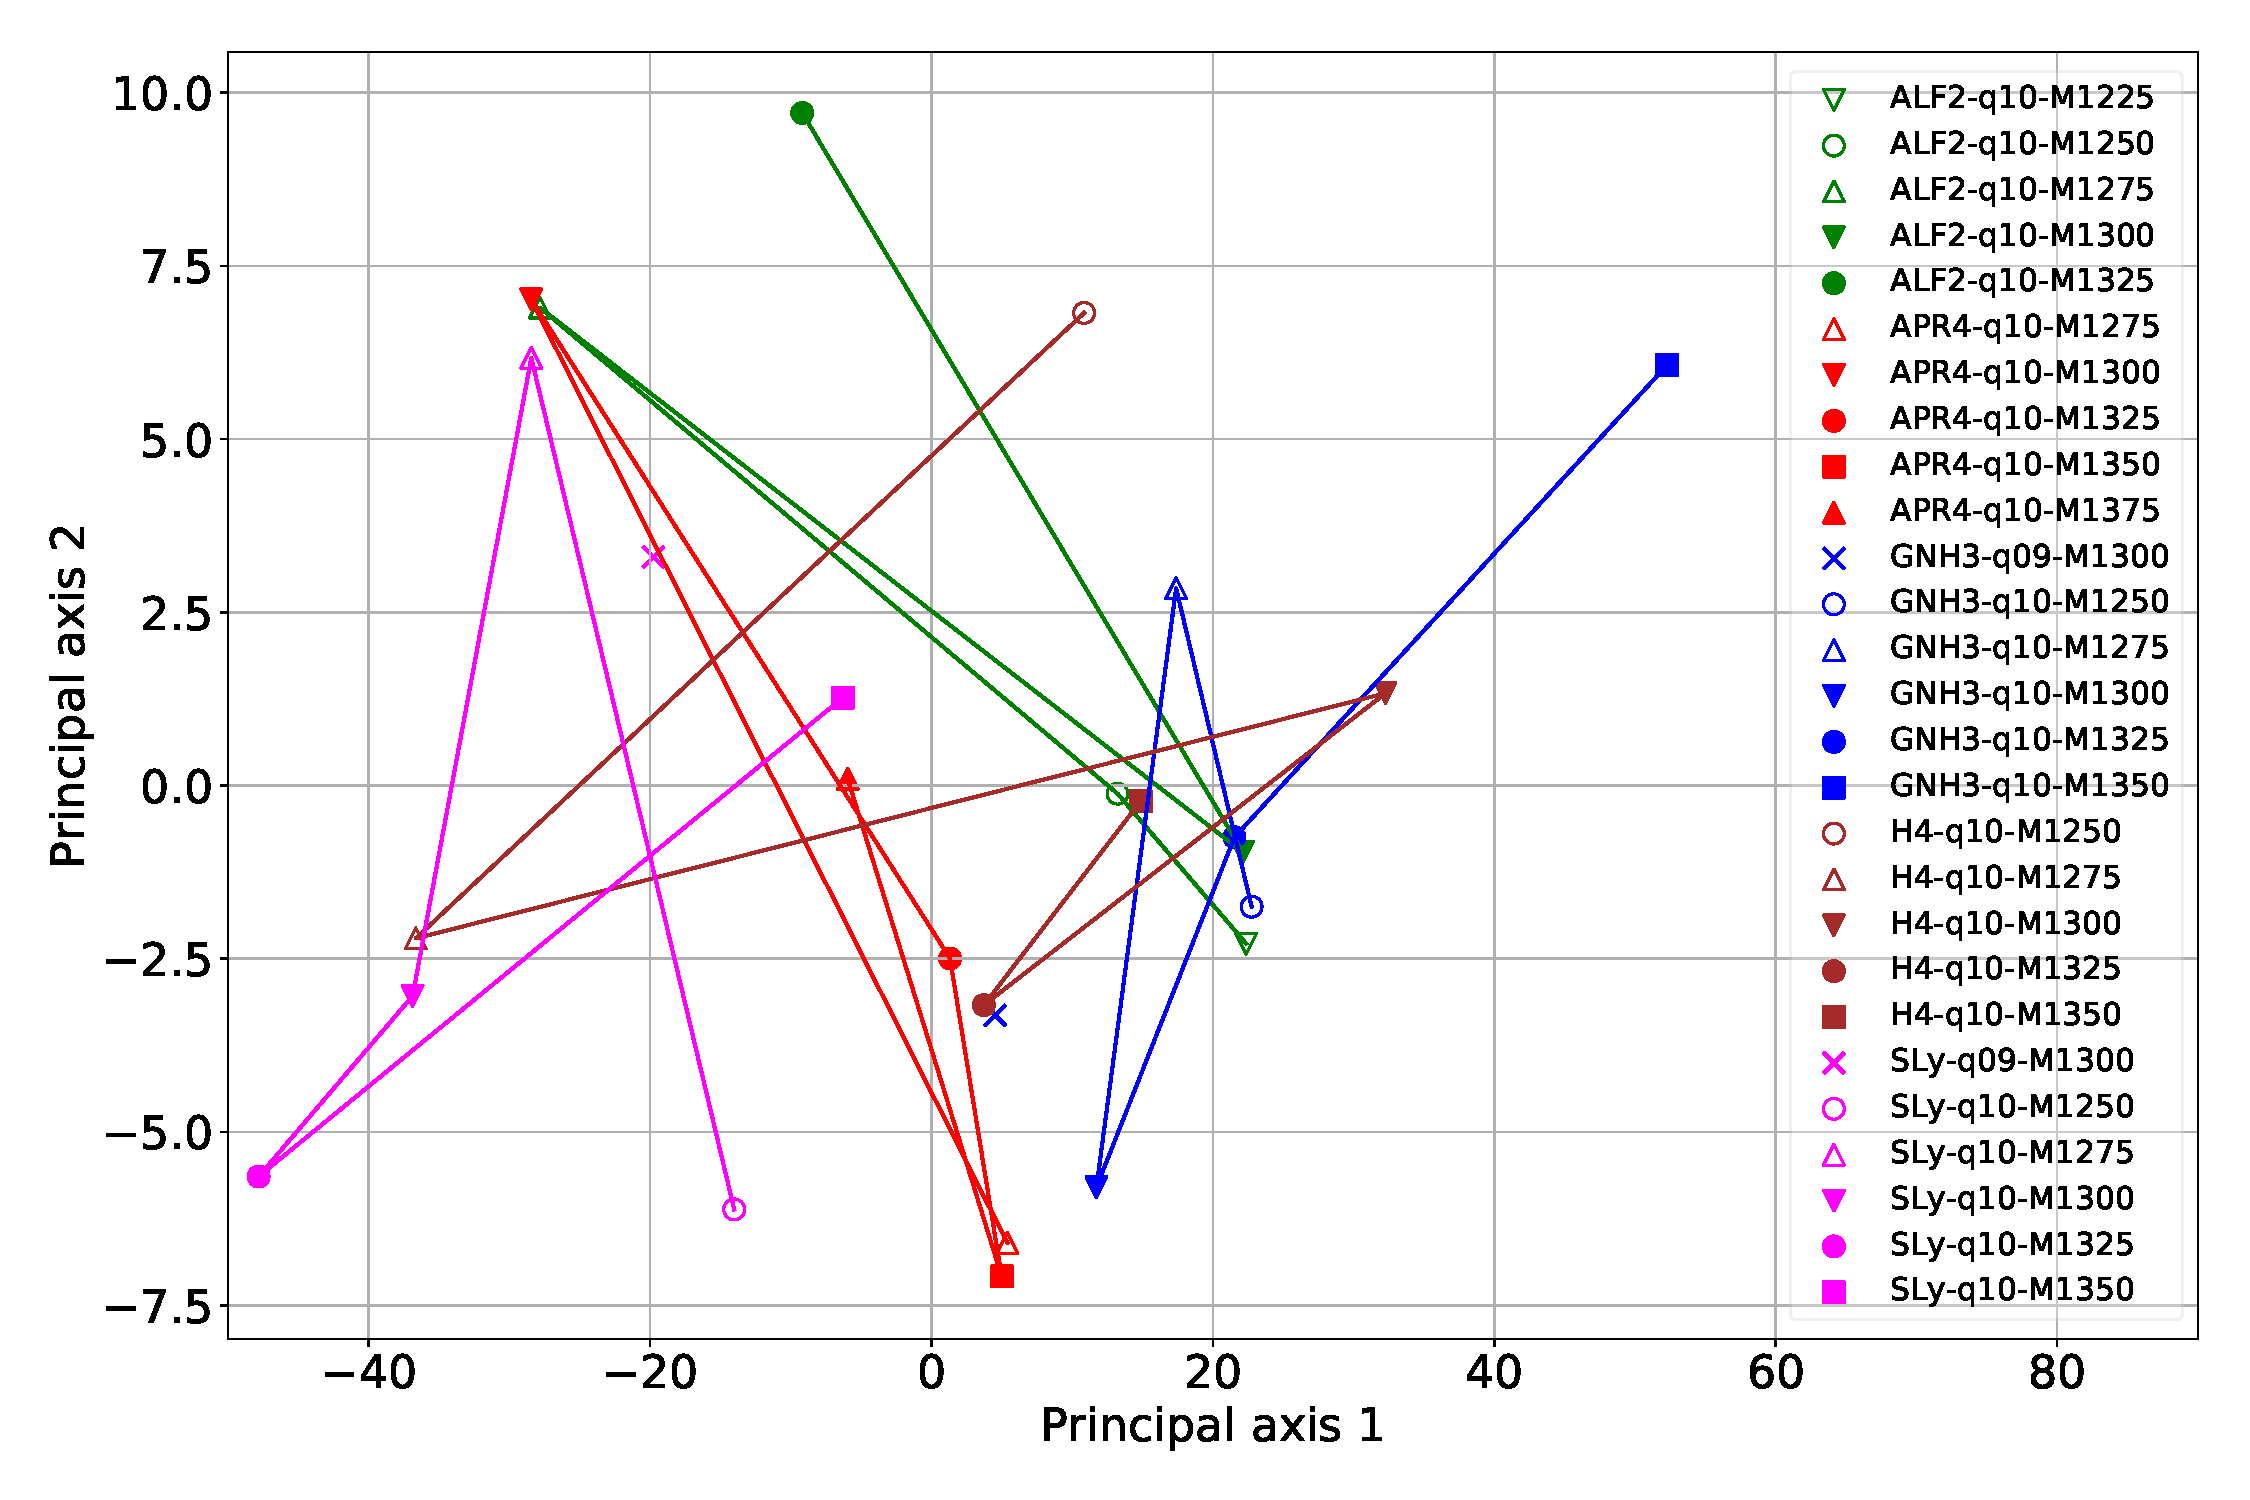
\includegraphics[width=15cm]{./img/PCAScaled2Dphase.pdf} 
	\caption[\protect\input{./img/PCAScaled2DphaseShort.txt}]{\protect\input{./img/PCAScaled2Dphase.txt}}
	\label{fig:PCAScaled2Dphase}
\end{figure}
A significant overlap is also shown in the XY projection of the PCA frequency scaled phase space, showing the difficulty in visually distinguishing between different EOS. It may be possible that the PCA decomposition without frequency scaling would be more insightful and this is investigated in the following section.\par

\subsubsection{Unscaled Frequency}
\label{sec:PCAUnscaled}
We generated a three component PCA decomposition of the unmodified Fourier transform of the waveform under test. Figure~\ref{fig:PCAUnscaled3Damp} shows the PCA response for the amplitude of the waveforms under test: 
\begin{figure}[H]
	\centering
	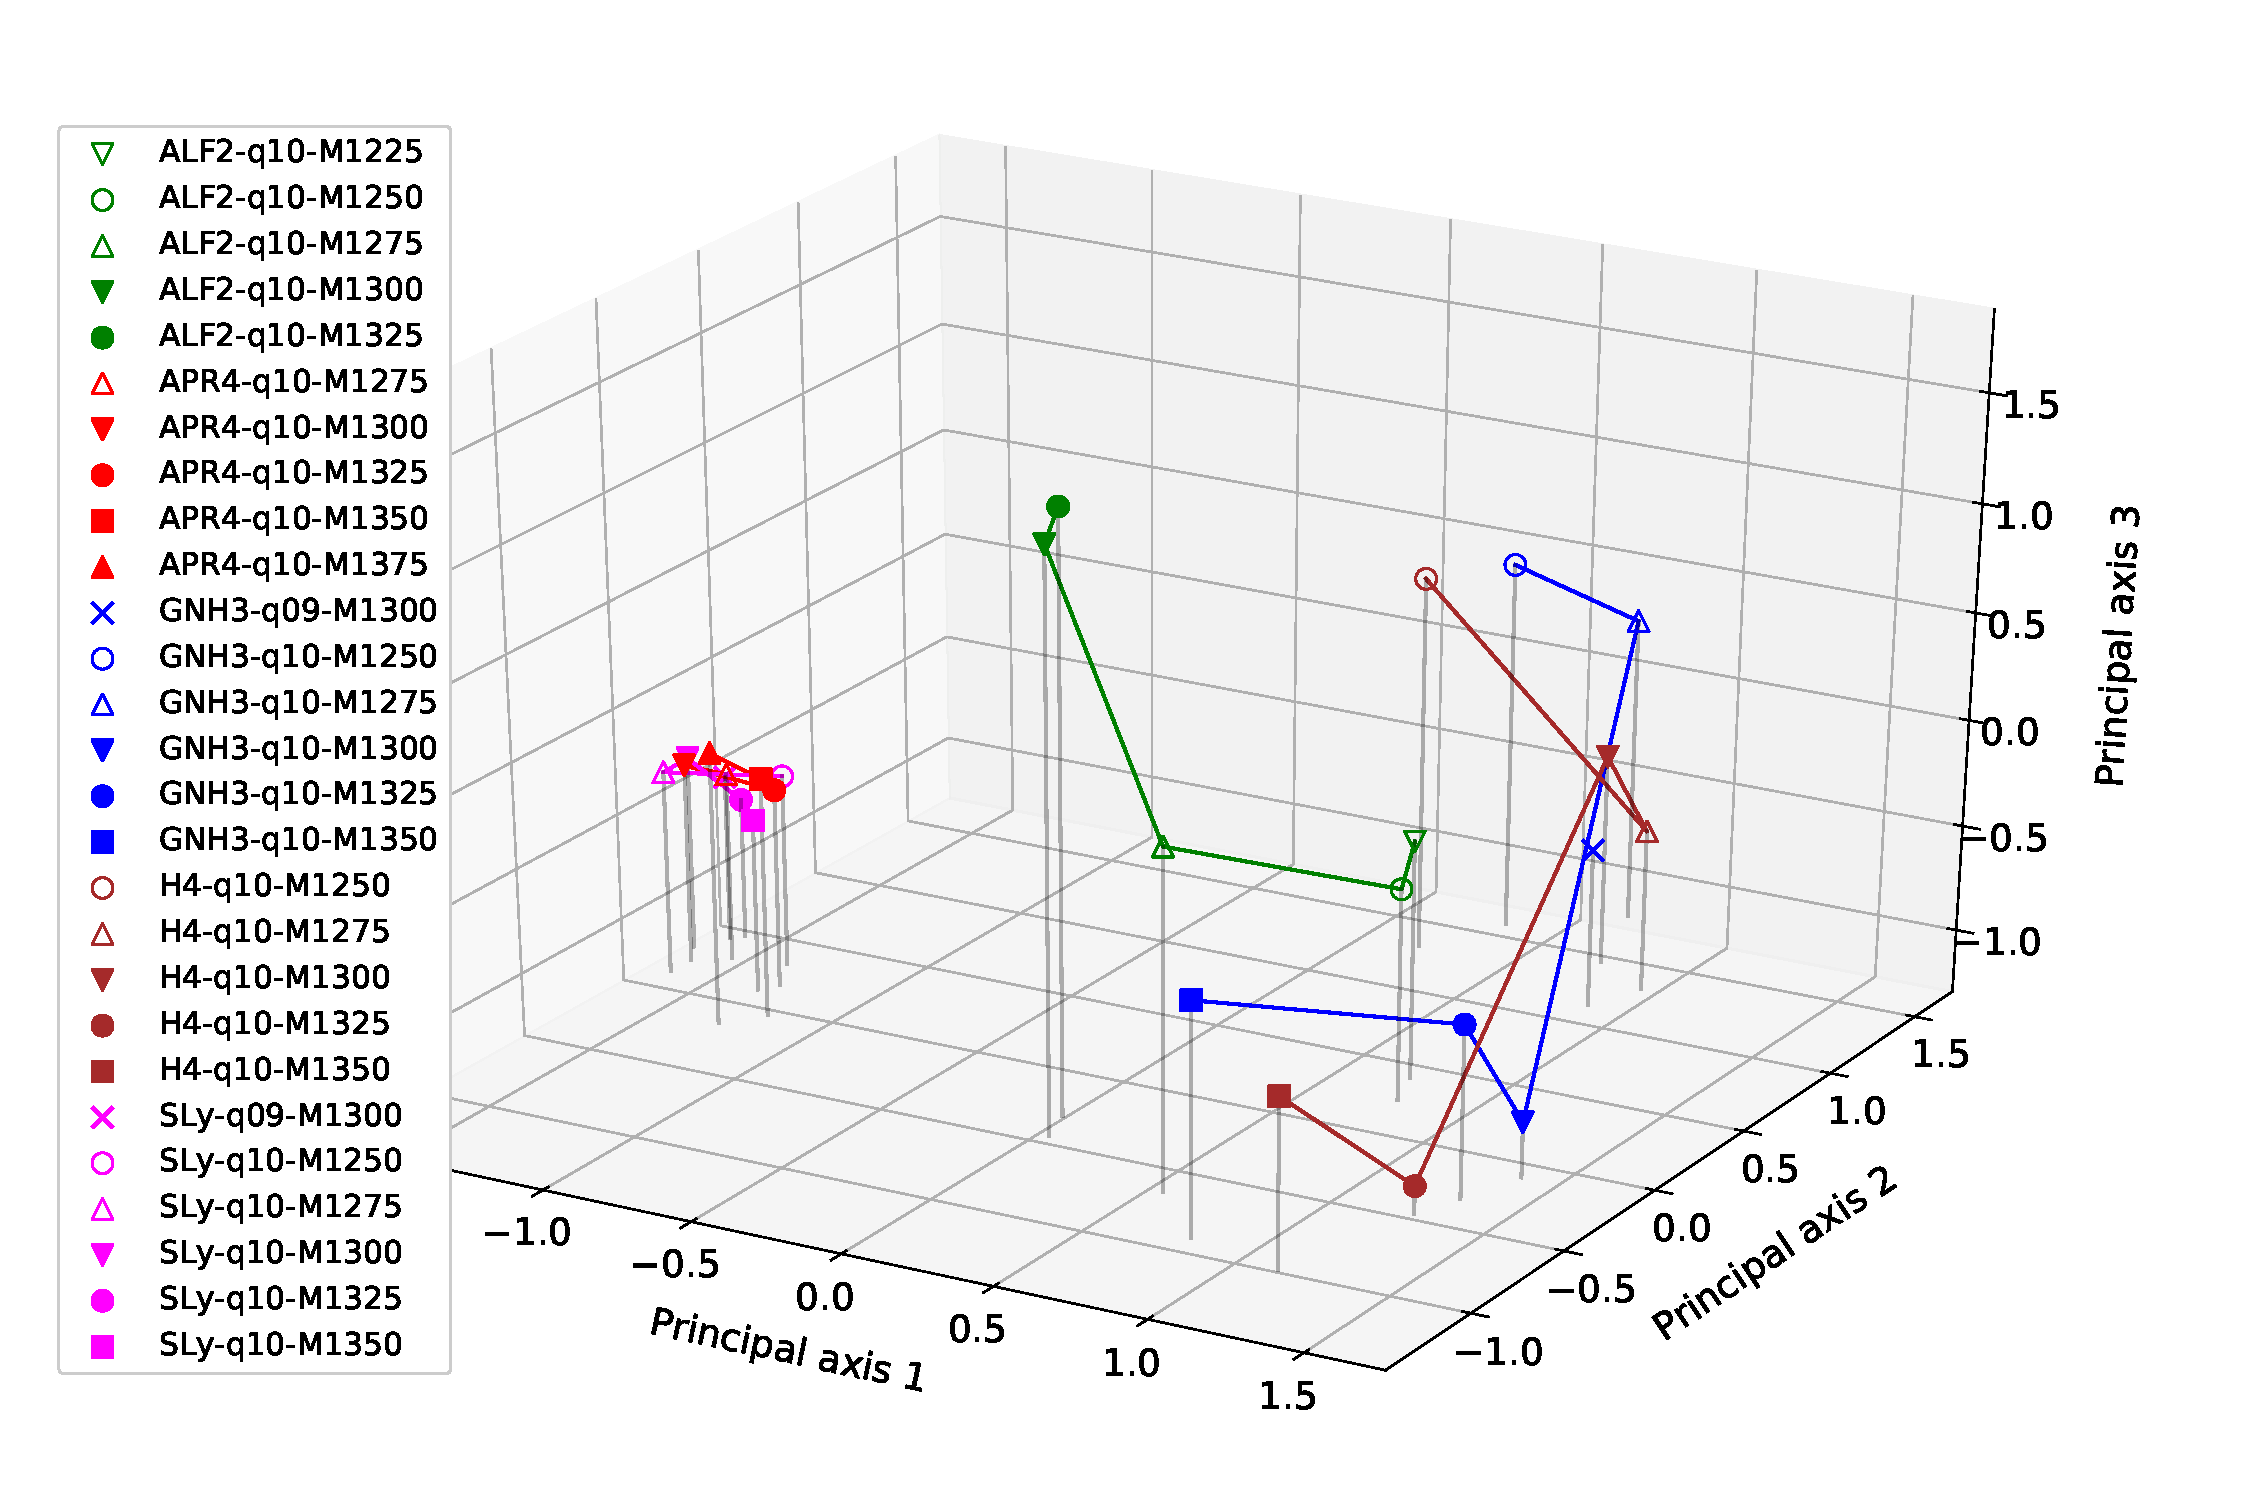
\includegraphics[width=15cm]{./img/PCAUnscaled3Damp.pdf} 
	\caption[\protect\input{./img/PCAUnscaled3DampShort.txt}]{\protect\input{./img/PCAUnscaled3Damp.txt}}
	\label{fig:PCAUnscaled3Damp}
\end{figure}
Without frequency scaling, there seems to be more separation of each EOS. This seems more promising as a potential input data-set for machine learning. There is still a tight clustering of the two EOS APR4 and SLy. However, if table~\ref{tbl:Waveforms2Table} is consulted, the strongest visual correlation between the first principal axis and peak frequency $f_{peak-j}$ with negative x values corresponding to high peak frequencies and vice versa.  This explains why this correlation is lost when frequency scaling occurs. Projecting the three dimensional PCA plot  down to the XY plane presents an even clearer picture of the PCA amplitude space:
\begin{figure}[H]
	\centering
	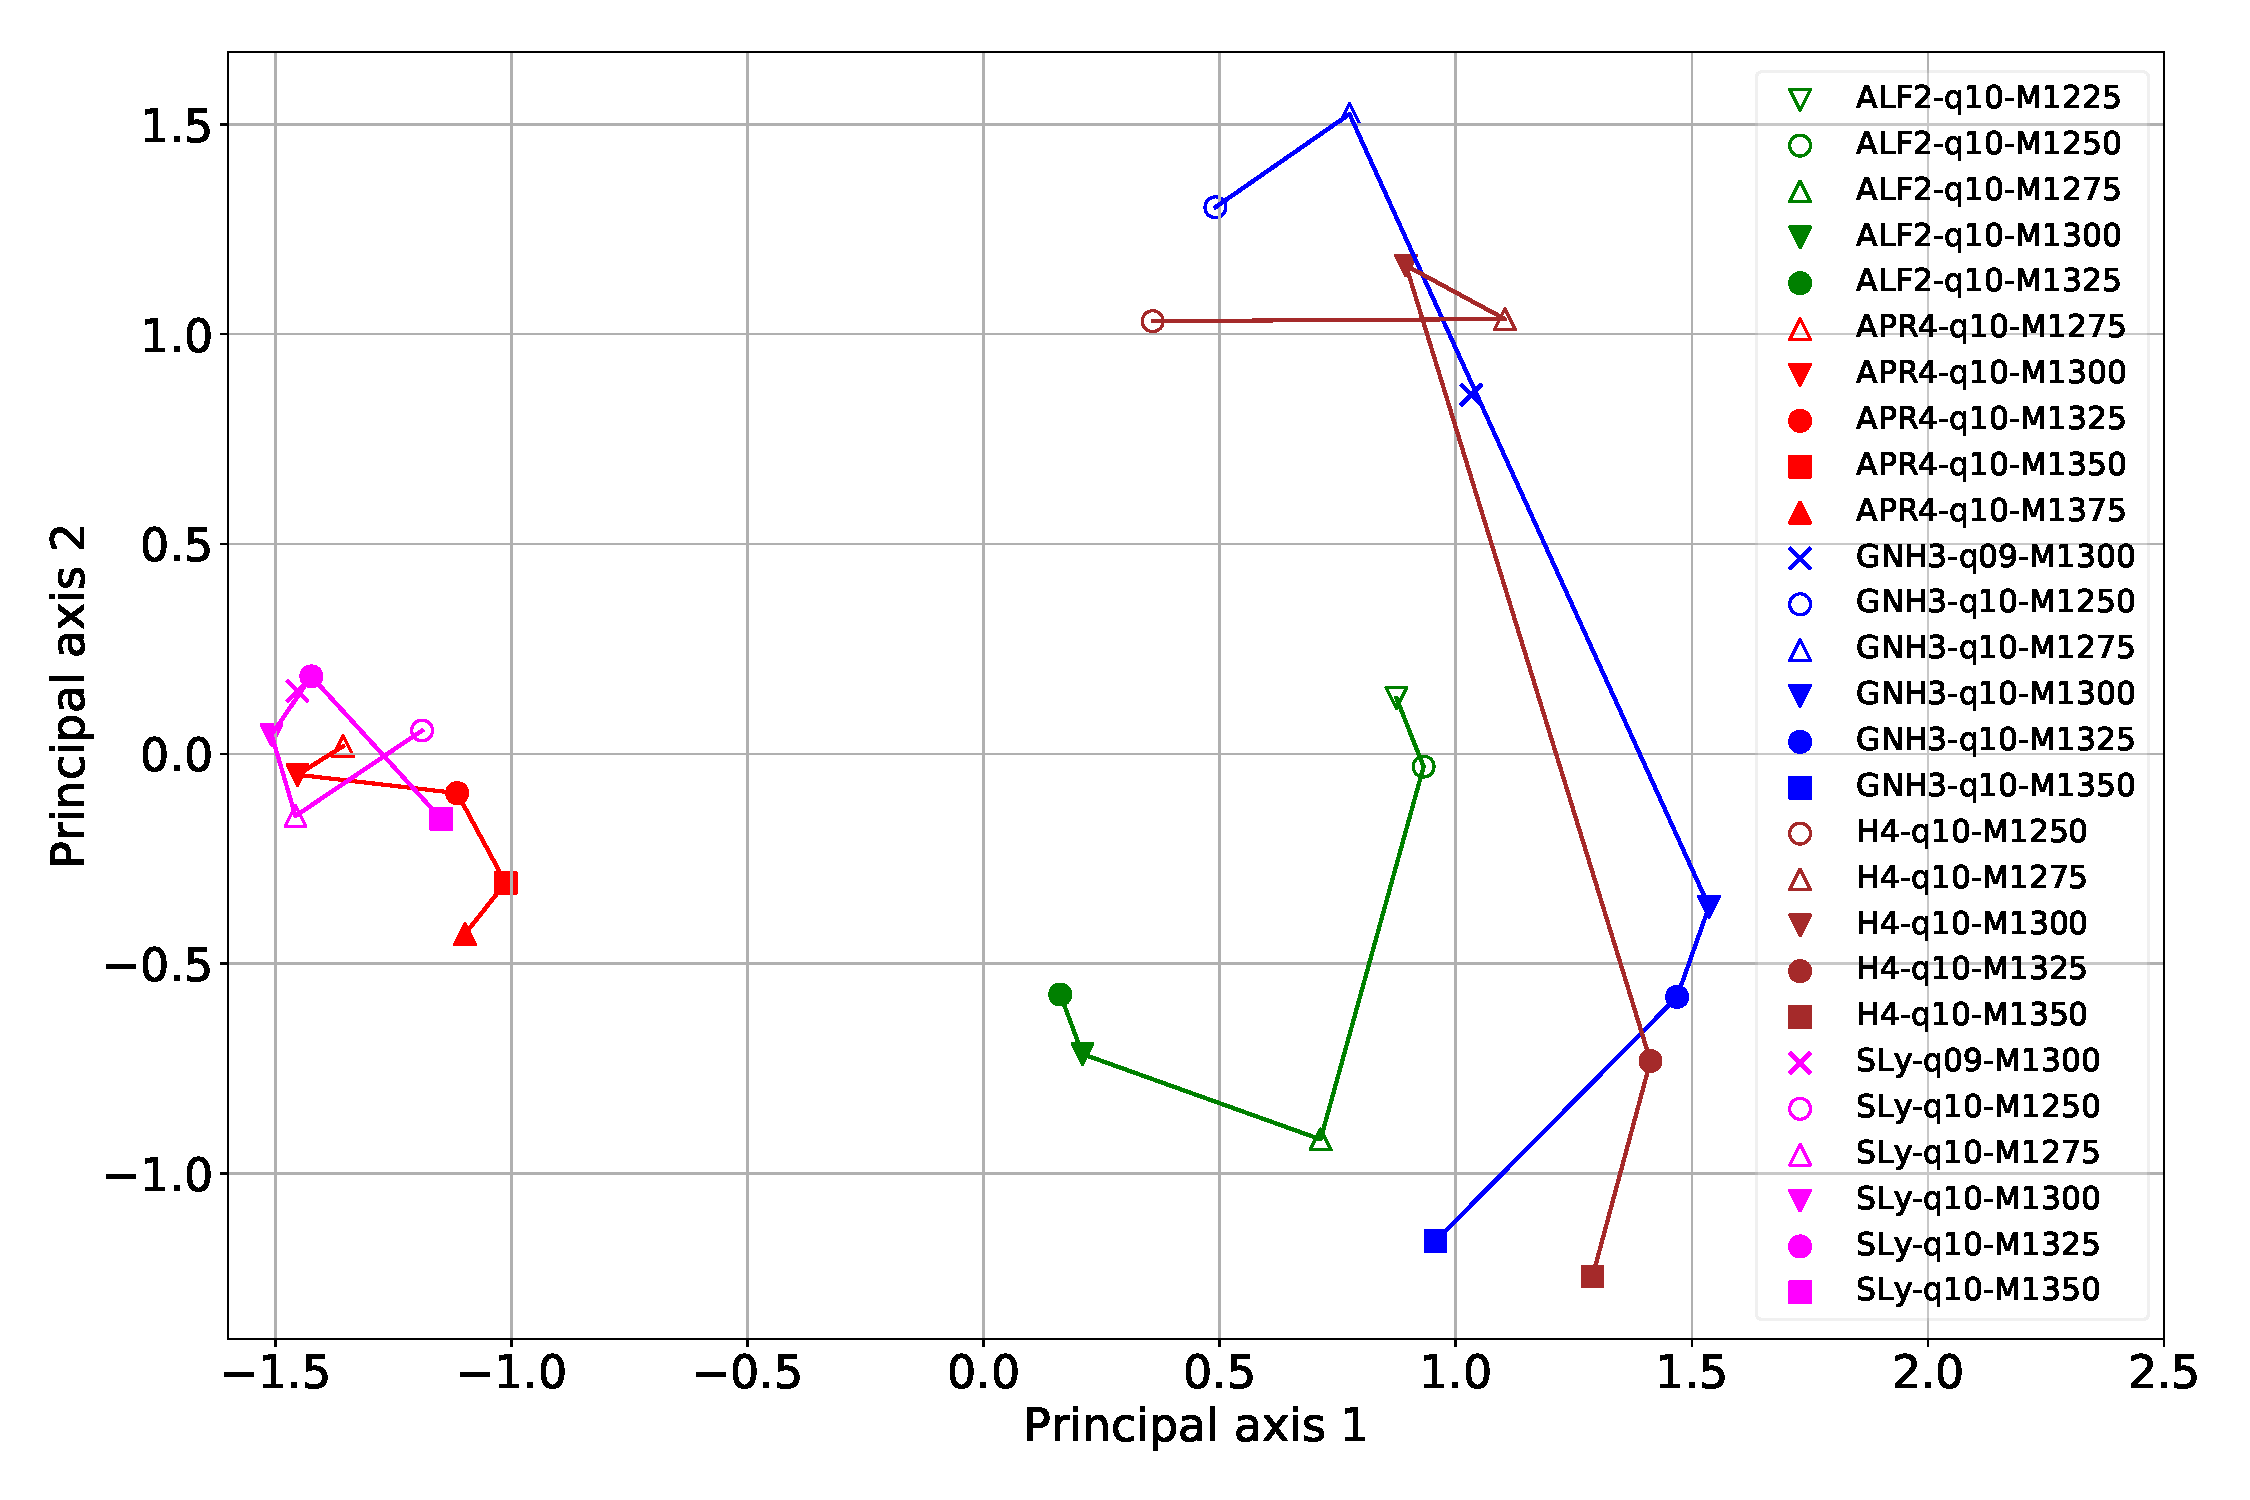
\includegraphics[width=15cm]{./img/PCAUnscaled2Damp.pdf} 
	\caption[\protect\input{./img/PCAUnscaled2DampShort.txt}]{\protect\input{./img/PCAUnscaled2Damp.txt}}
	\label{fig:PCAUnscaled2Damp}
\end{figure}
The large gap observed in the PCA space between the EOS APR4/SLy and ALF2/GNH3/H4 seems to correspond mainly to differences in peak frequency and to a lesser degree the compactness, and other tidal parameters. It should also be noted that \cite{Bernuzzi2015} developed a relationship between $f_{\text{peak}}$, the average mass ($\bar{\text{M}}$), and the tidal parameter ($\kappa^T_2$), indicating that it may be possible to eliminate $f_{\text{peak}}$ as a parameter by using the tidal parameters instead. This is preferable for the unscaled frequency system, as it means that there is no pre-processing involved. Looking now at the  the phase response for the unscaled waveforms as shown in figure~\ref{fig:PCAUnscaled3Dphase}:
\begin{figure}[H]
	\centering
	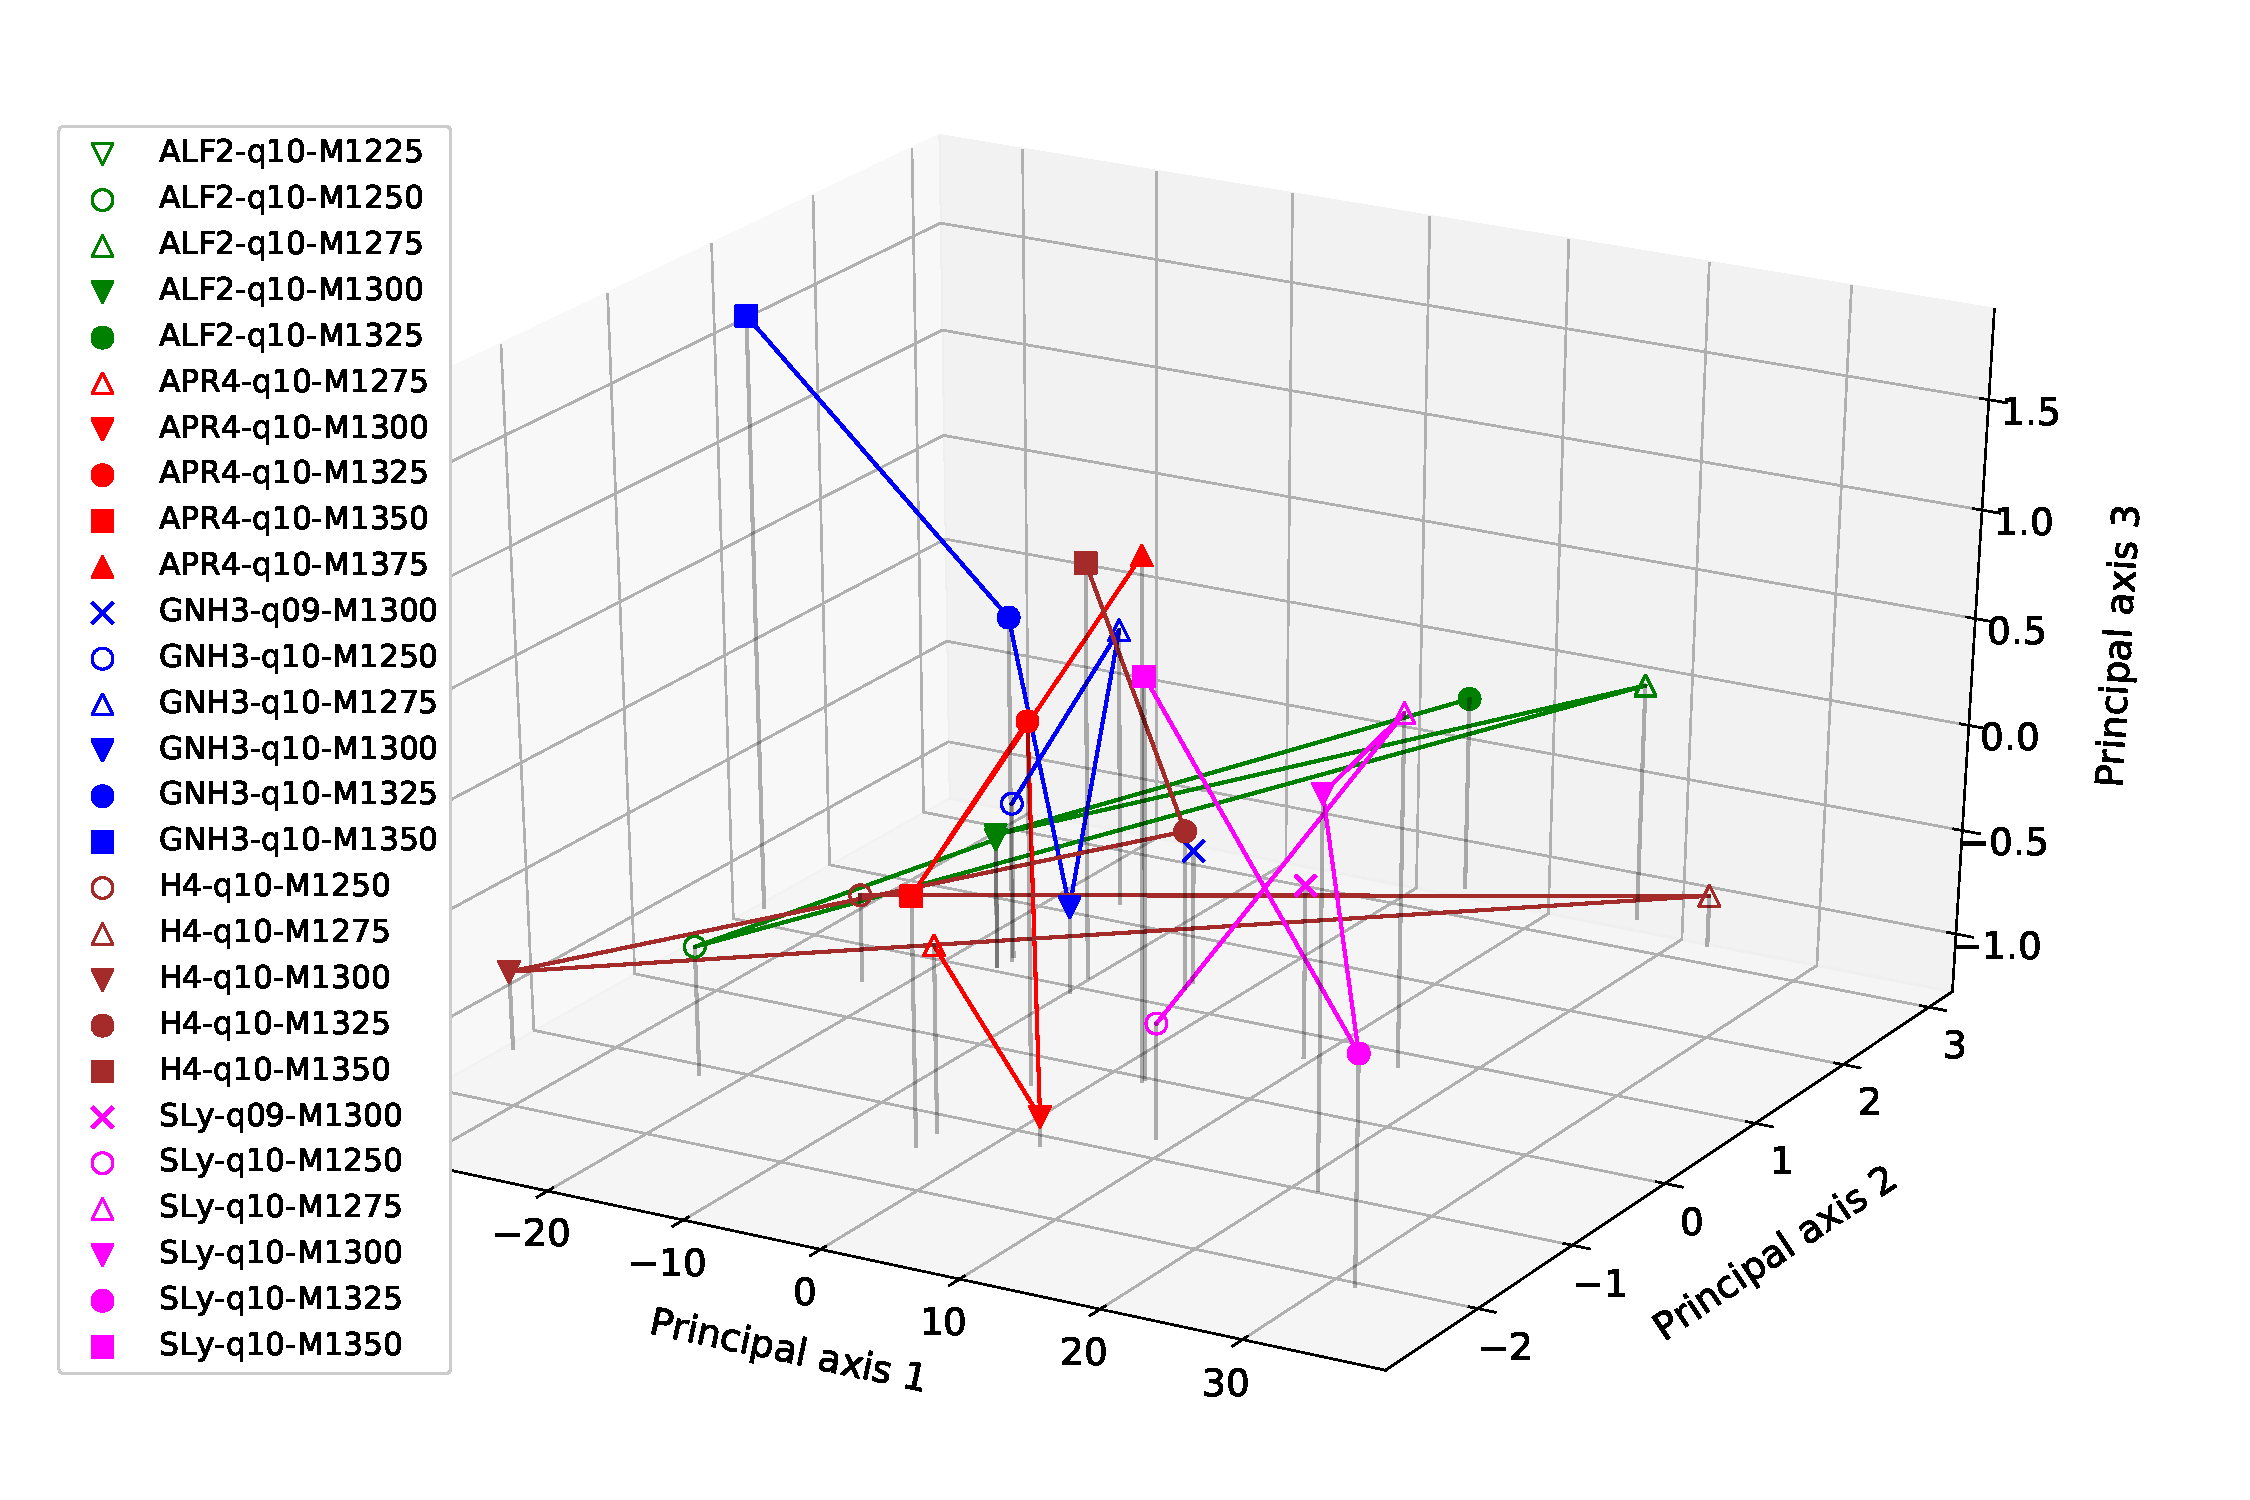
\includegraphics[width=15cm]{./img/PCAUnscaled3Dphase.pdf} 
	\caption[\protect\input{./img/PCAUnscaled3DphaseShort.txt}]{\protect\input{./img/PCAUnscaled3Dphase.txt}}
	\label{fig:PCAUnscaled3Dphase}
\end{figure}
The phase response looks quite tangled, as with the scaled response in figure~\ref{fig:PCAScaled3Damp}, so projection to the XY plane was performed to give figure~\ref{fig:PCAUnscaled2Dphase}:
\begin{figure}[H]
	\centering
	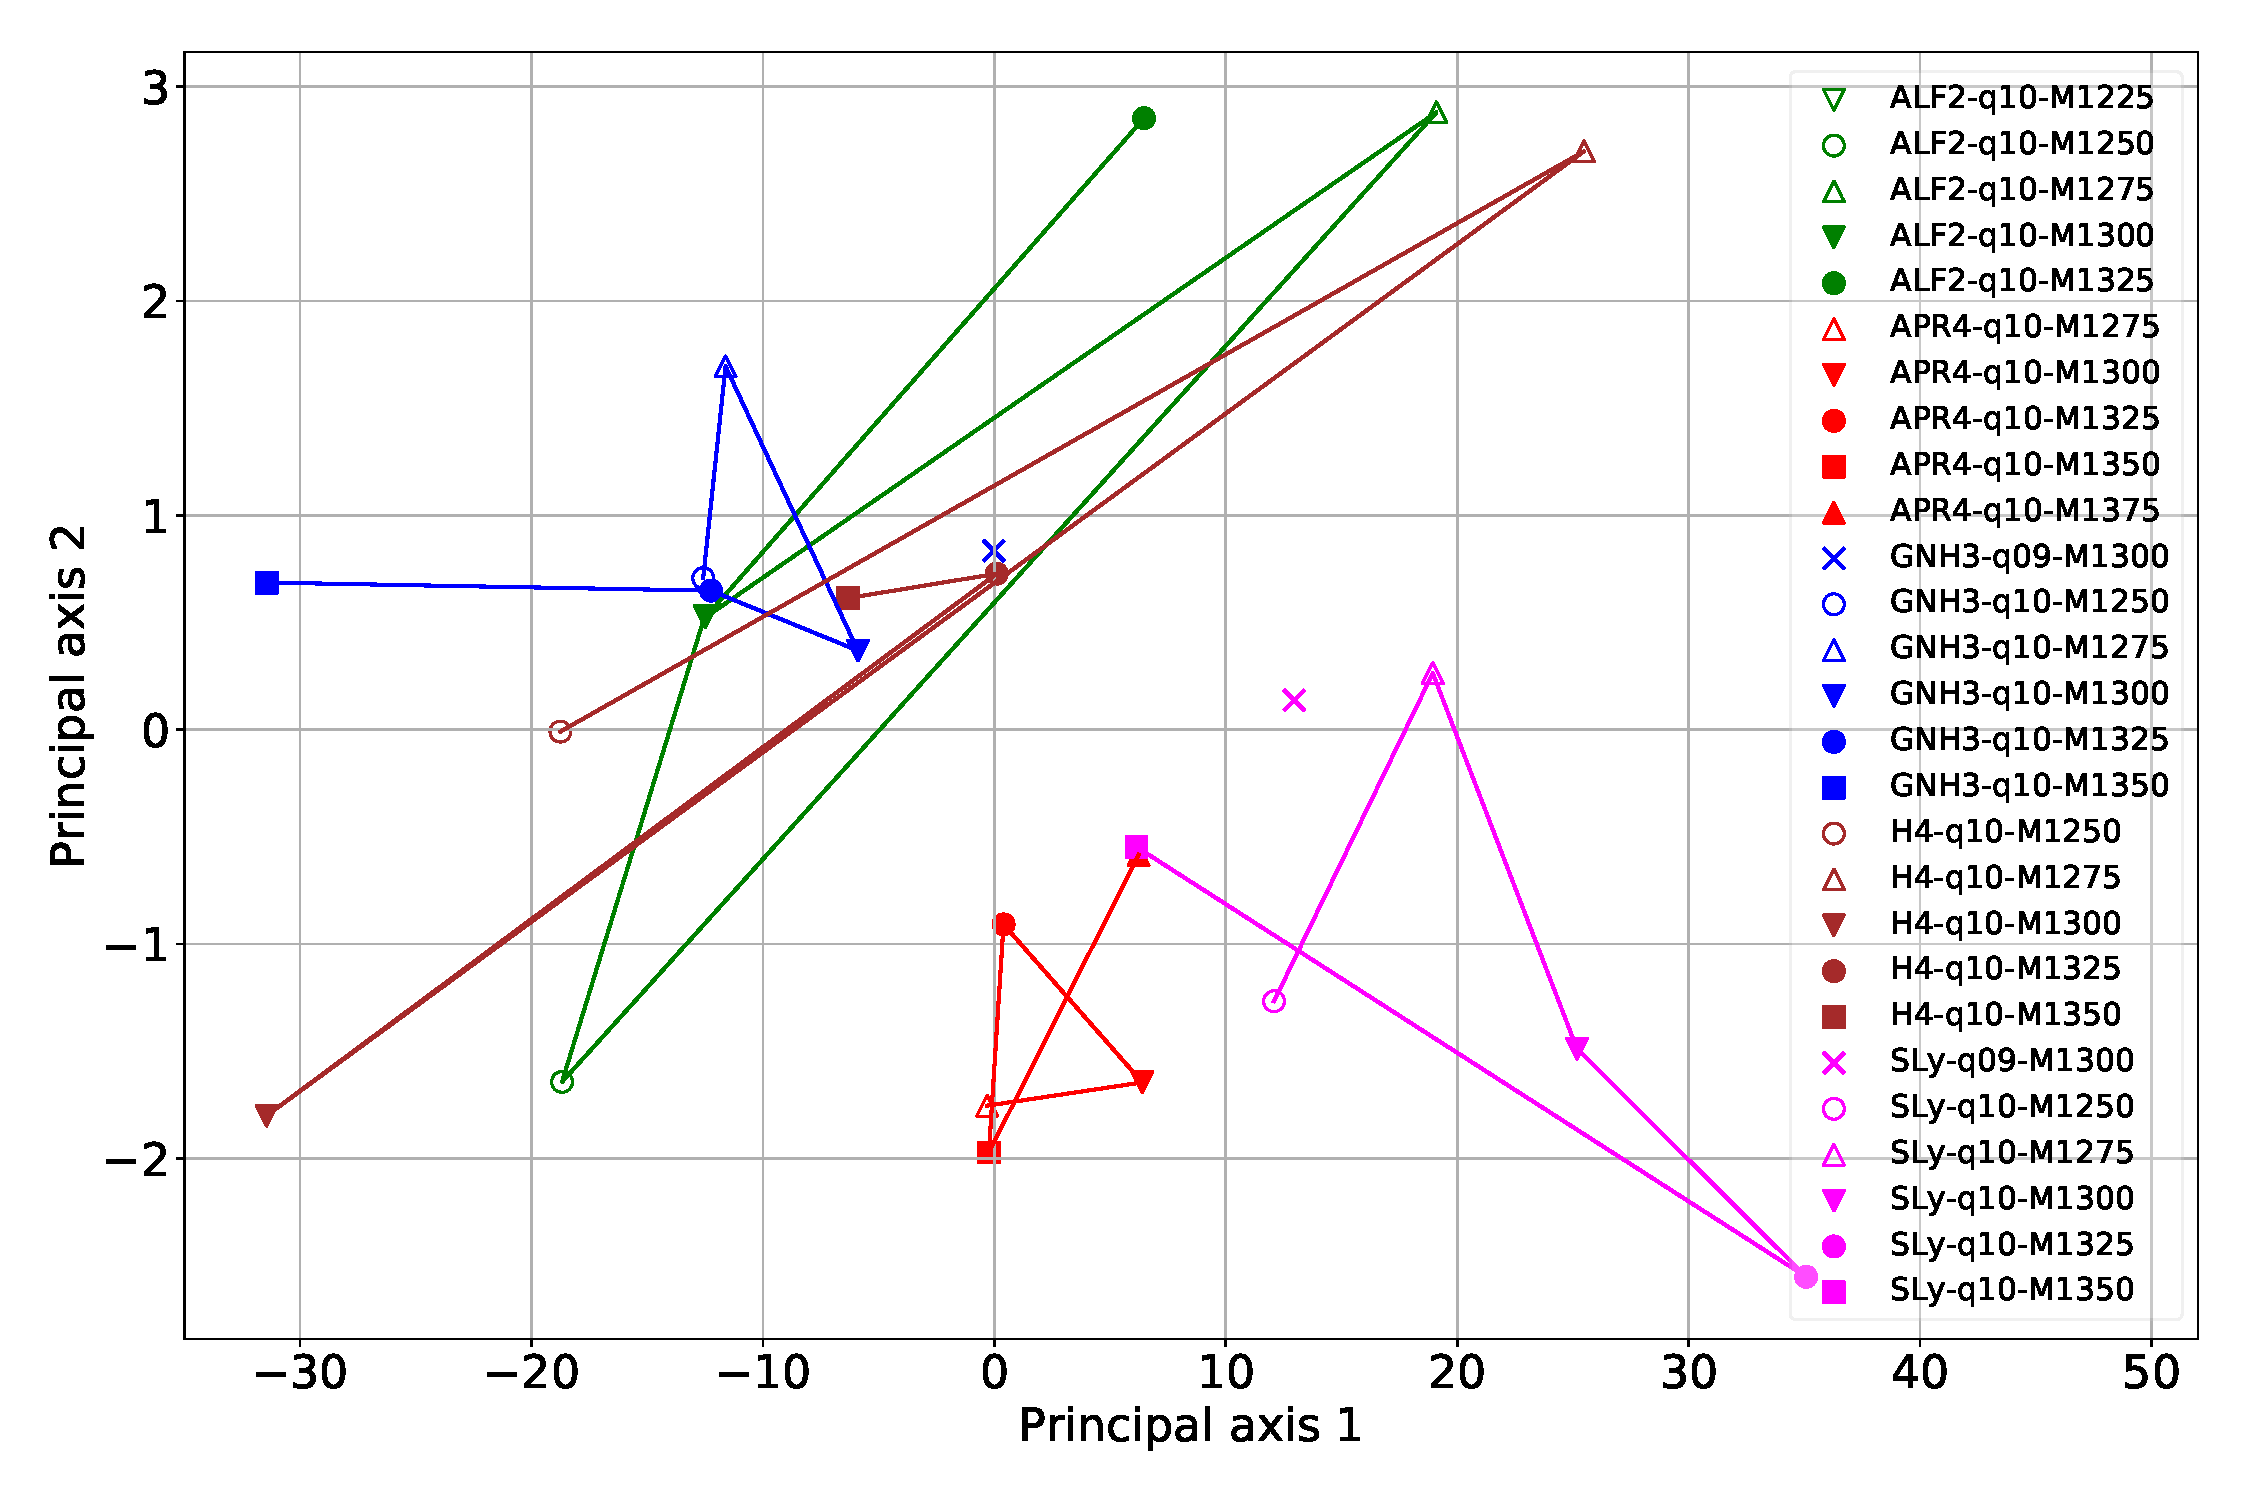
\includegraphics[width=15cm]{./img/PCAUnscaled2Dphase.pdf} 
	\caption[\protect\input{./img/PCAUnscaled2DphaseShort.txt}]{\protect\input{./img/PCAUnscaled2Dphase.txt}}
	\label{fig:PCAUnscaled2Dphase}
\end{figure}
Here we can still clearly see a distinction between the APR4/SLy and ALF2/GNH3/H4 equation of states which was not visible in three dimensional PCA space suggesting that a machine learning algorithm would be better using the unscaled Fourier spectra. 
\subsubsection{Principal components summary}
The PCA analysis on both the scaled and unscaled frequency values for the Fourier transform of the waveforms suggests that a learning algorithm may be more successful using the unscaled frequency values for the FFT of the gravitational-wave strain signals rather than the frequency scaled data. This is examined in section~\ref{sec:TheCannon}.

\subsection{The Cannon analysis}
\label{sec:TheCannon}
The Cannon 2 implementation was setup as described in section~\ref{sec:TheCannonSetup} and the waveforms have been restricted to equal mass systems with the EOS GAM2 excluded. I have also selected two waveforms to use as example signals: APR4 EOS, with an average mass of 1.275M$_\odot$, and ALF2 EOS with average mass of 1.225M$_\odot$. There has been no frequency scaling for analysis performed using the Cannon algorithm. The following plots show the amplitude of the Fourier transform multiplied by the square root of the frequency as this value is often used in numerical relativity \citep[eg][]{Clark2015, Takami2015} because it can be directly compared with the LIGO amplitude spectral density. 
\subsubsection{Entire training set}
\label{sec:TheCannonEntireTrainingSet}
The entire training set was used for this section and leave one out cross-validation was performed in section~\ref{sec:TheCannonLOOCV}. Figure~\ref{fig:CannonLogAmpPhAPR4-q10-M1275} shows the response generated from APR4 EOS with a mean mass of 1.275M$_\odot$ using the Cannon algorithm.
\begin{figure}[H]
	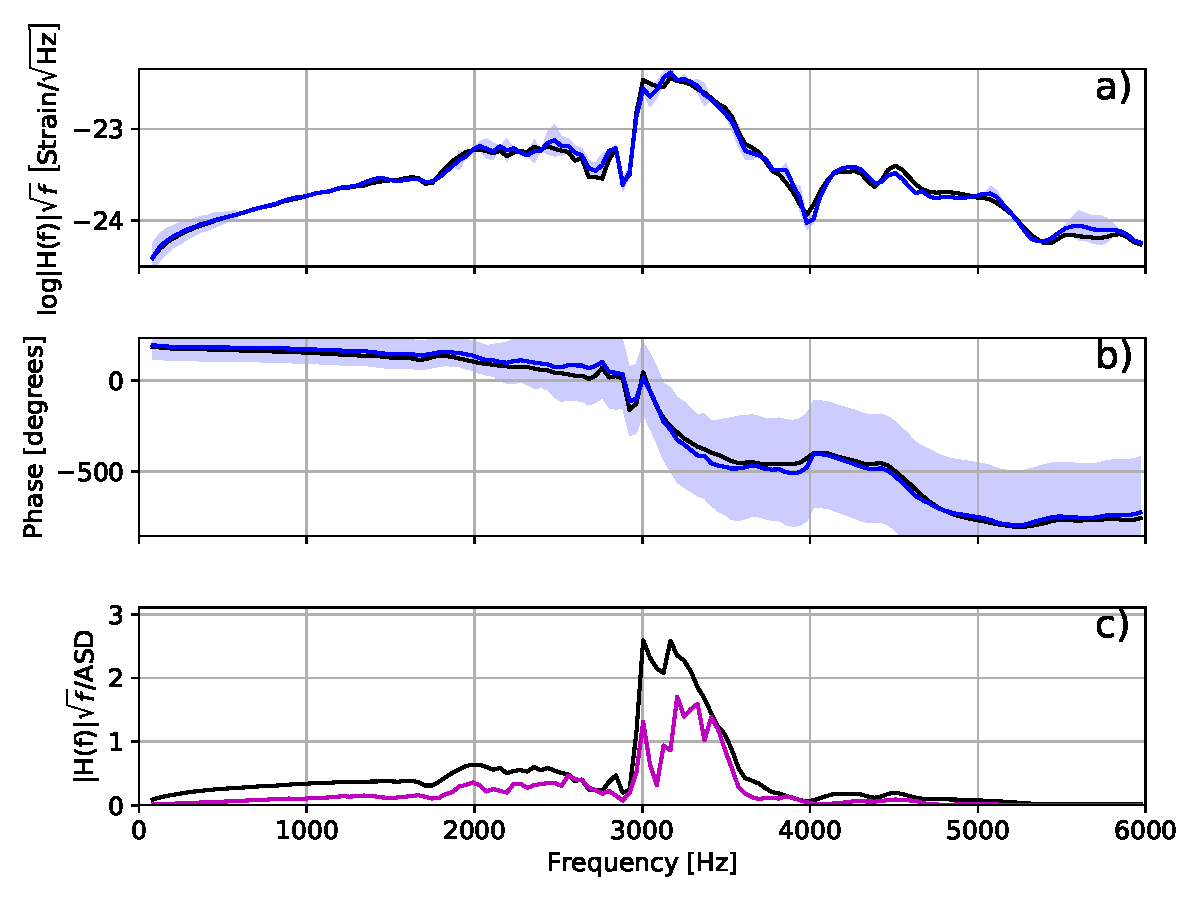
\includegraphics[width=15cm]{./img/CannonLogAmpPhAPR4-q10-M1275.pdf} 
	\caption[\protect\input{./img/CannonLogAmpPhAPR4-q10-M1275Short.txt}]{\protect\input{./img/CannonLogAmpPhAPR4-q10-M1275.txt}}
	\label{fig:CannonLogAmpPhAPR4-q10-M1275}
\end{figure}

The total SNR for this signal is 2.06 and the residual SNR was 1.10. The goal of the residual SNR plots is to achieve a number significantly less than one, this is to ensure that the reconstructed waveform is indistinguishable . Plot a) shows the amplitude response of APR4/1.275M$_\odot$ scaled by the square root of the frequency in log based 10 units. The black trace is the original FFT amplitude of the signal, and the blue trace is the reconstructed signal determined by the learning algorithm. Plot b) shows the phase response in degrees with black trace referring to the phase of the original FFT, and the blue trace referring to the reconstructed phase of the FFT, generated by The Cannon model. The shaded blue area in both of these plots indicate the uncertainty in the amplitude or phase of the model. Plot c) gives an indication of the errors in the reconstructed signal, where the error in the signal is given by the complex difference between the original signal and the reconstructed signal. The black trace shows $\zeta(h,f)$,  the significance of the original signal for a given frequency (equation~\ref{eq:zetah}). The pink trace $\zeta(\Delta h,f)$ (equation~\ref{eq:zetadeltah}) shows the significance of the error in the reconstructed waveform for a given frequency. For this waveform, the error of the signal is around half the signal strength. Figure~\ref{fig:CannonLogAmpPhALF2-q10-M1225} shows the corresponding response of ALF2/1.225M$_\odot$. 
\begin{figure}[H]
	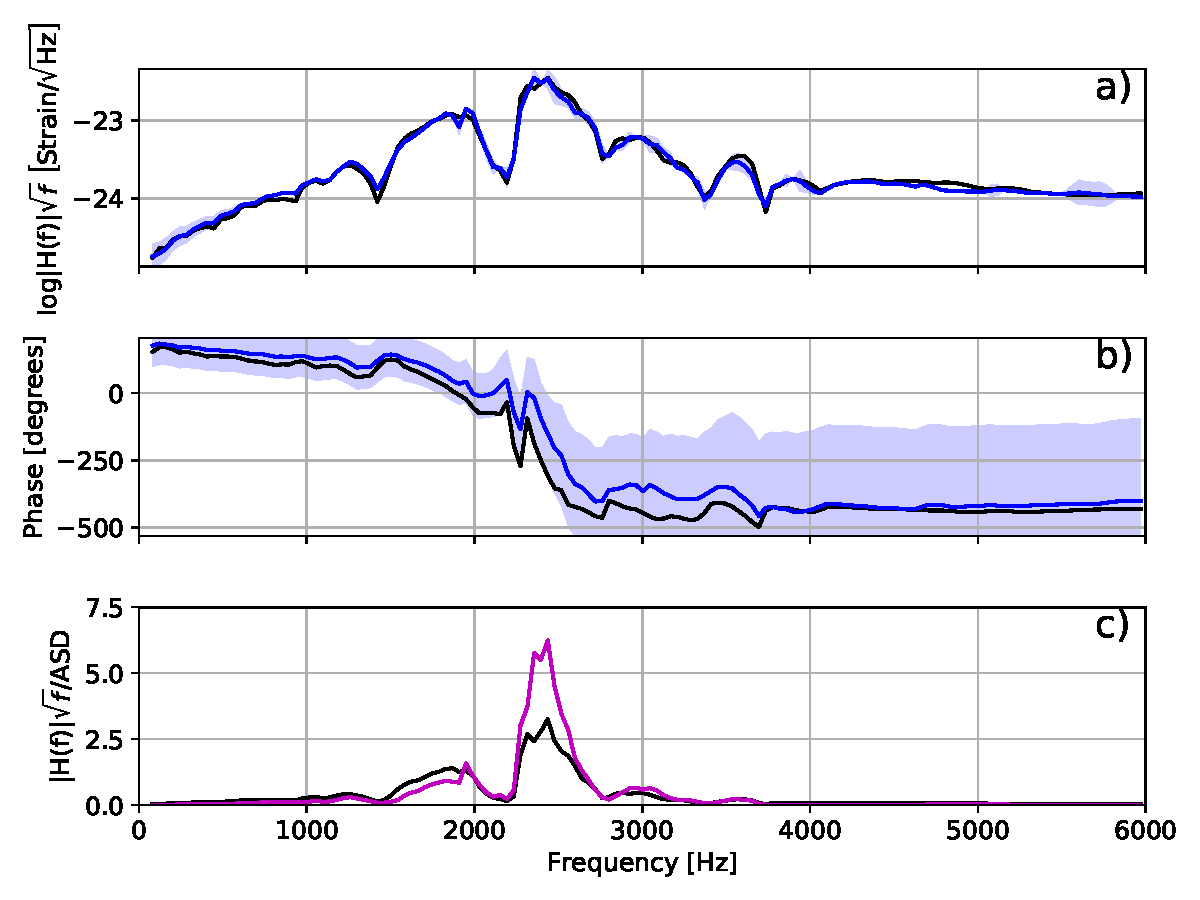
\includegraphics[width=15cm]{./img/CannonLogAmpPhALF2-q10-M1225.pdf} 
	\caption[\protect\input{./img/CannonLogAmpPhALF2-q10-M1225Short.txt}]{\protect\input{./img/CannonLogAmpPhALF2-q10-M1225.txt}}
	\label{fig:CannonLogAmpPhALF2-q10-M1225}
\end{figure} 
The SNR for this signal is 2.33 and the residual SNR was 3.56. Looking at plot c) it can be seen that the maximum error occurs around the maximum amplitude. The amplitude in plot~a) looks fairly close to the original signal, however the \textit{phase} is off by around 180 degrees, which is consistent with an error value of twice the original signal, as observed in the pink plot of $\zeta(\Delta h,f)$. The residual SNR for this signal is too high even though the waveform under test was included in the training set. However, cross-validation is required to get a complete picture of the performance of this method as is investigated in the following section. 
\subsubsection{Leave one out cross-validation}
\label{sec:TheCannonLOOCV}
Figures~\ref{fig:CannonLogAmpPhALF2-q10-M1225}~and~\ref{fig:CannonLogAmpPhAPR4-q10-M1275} are not true cross-validation waveforms. Although the waveform parameters are inferred from the learning mode, the signals under test were included in the training set. To perform leave one out cross-validation (see section~\ref{sec:CrossValidation}), the signals under test should be excluded from the training set, as performed in this section. Figure~\ref{fig:CannonLogAmpPhAPR4-q10-M1275-cv} shows the cross-validation waveform for APR4/1.275M$_\odot$:
\begin{figure}[H]
	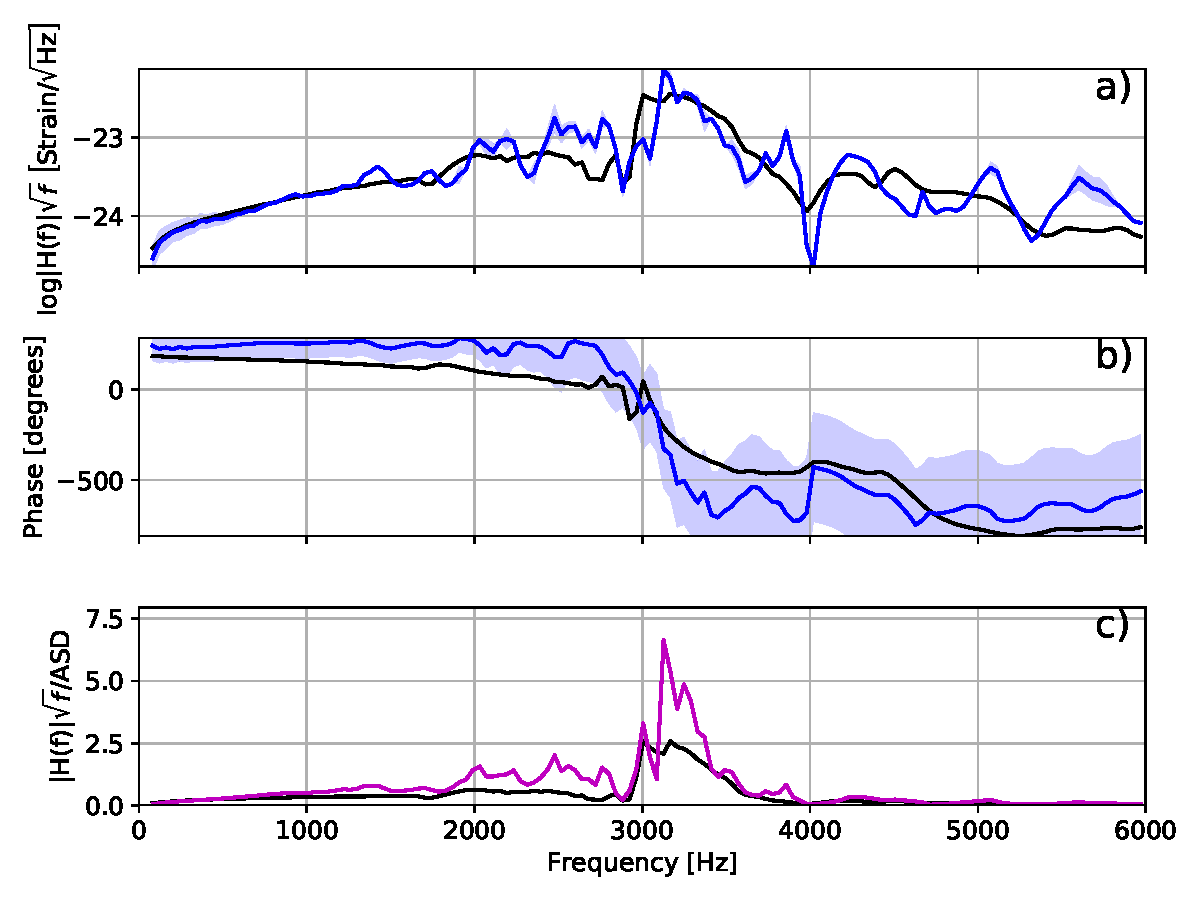
\includegraphics[width=15cm]{./img/CannonLogAmpPhAPR4-q10-M1275-cv.pdf} 
	\caption[\protect\input{./img/CannonLogAmpPhAPR4-q10-M1275Short-cv.txt}]{\protect\input{./img/CannonLogAmpPhAPR4-q10-M1275-cv.txt}}
	\label{fig:CannonLogAmpPhAPR4-q10-M1275-cv}
\end{figure}
The residual SNR for this waveform is now 3.63, compared to 1.10 without cross-validation (figure~\ref{fig:CannonLogAmpPhAPR4-q10-M1275}), so it is clear that leave one out cross-validation causes significant deterioration in the residual SNR. This could potentially be explained by the small quantity of waveforms within the training set. Cross-validation is often performed with 30\% of the waveforms used as the test set, and the remaining 70\% of the waveforms used for the training set. This is not an option when there are only 25 waveforms to start with, and clearly, even leaving one waveform out results in poor training in this situation. The second waveform under test is shown in \ref{fig:CannonLogAmpPhALF2-q10-M1225-cv}:
\begin{figure}[H]
	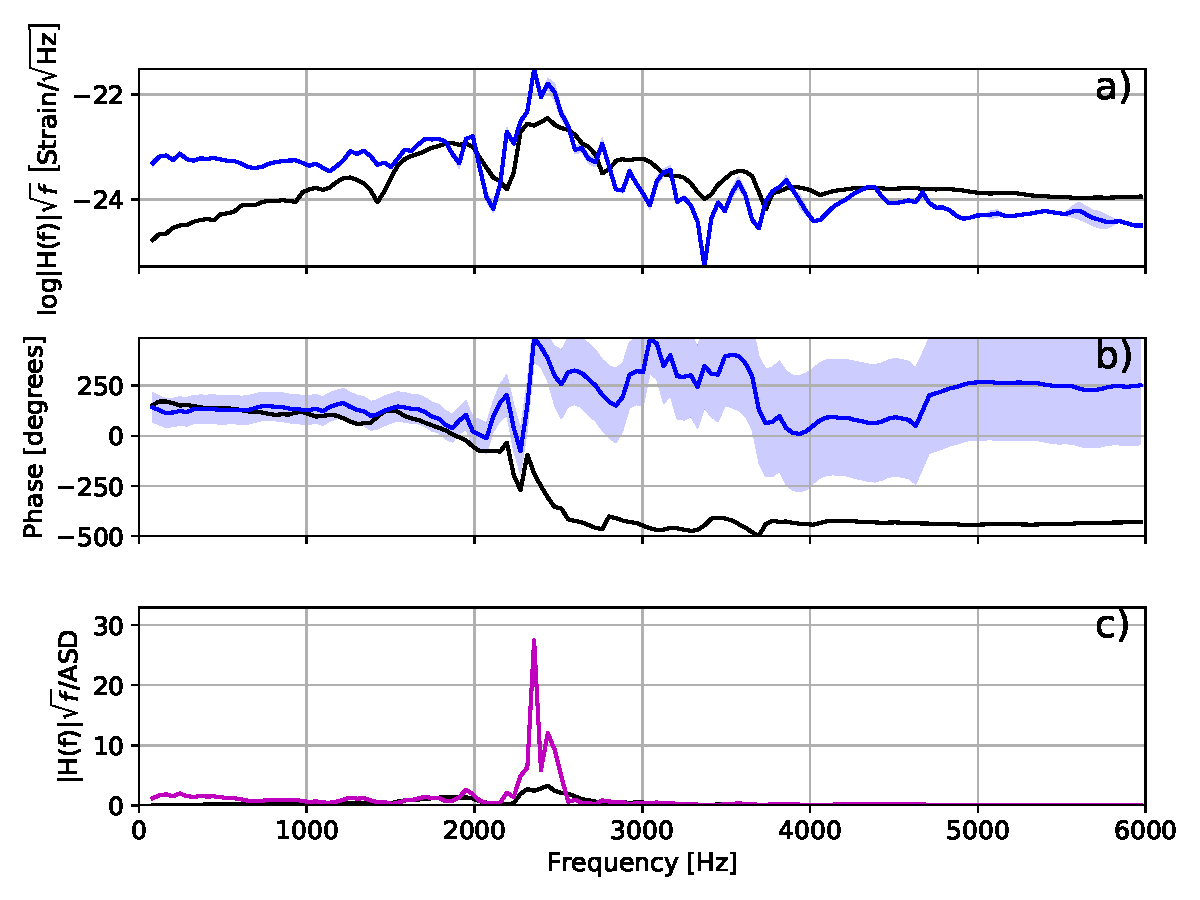
\includegraphics[width=15cm]{./img/CannonLogAmpPhALF2-q10-M1225-cv.pdf} 
	\caption[\protect\input{./img/CannonLogAmpPhALF2-q10-M1225Short-cv.txt}]{\protect\input{./img/CannonLogAmpPhALF2-q10-M1225-cv.txt}}
	\label{fig:CannonLogAmpPhALF2-q10-M1225-cv}
\end{figure}
The deterioration in the residual SNR is more extreme, going from 3.56 (in figure~\ref{fig:CannonLogAmpPhALF2-q10-M1225}) to 10.05 in this figure. The amplitude deviates significantly around the peak of the waveform, resulting in a large error term of around 28 as can be seen in the pink curve on plot~c). Using a sample of two waveforms from 25 does not give the overall picture, it may be that these two waveforms are better or worse than the rest and are not a representative sample. A histogram of residual SNR was generated for all leave one out cross-validation waveforms for The Cannon and is shown in figure~\ref{fig:CannonLogAmpPh-hist-cv}.  
\begin{figure}[H]
	\centering
	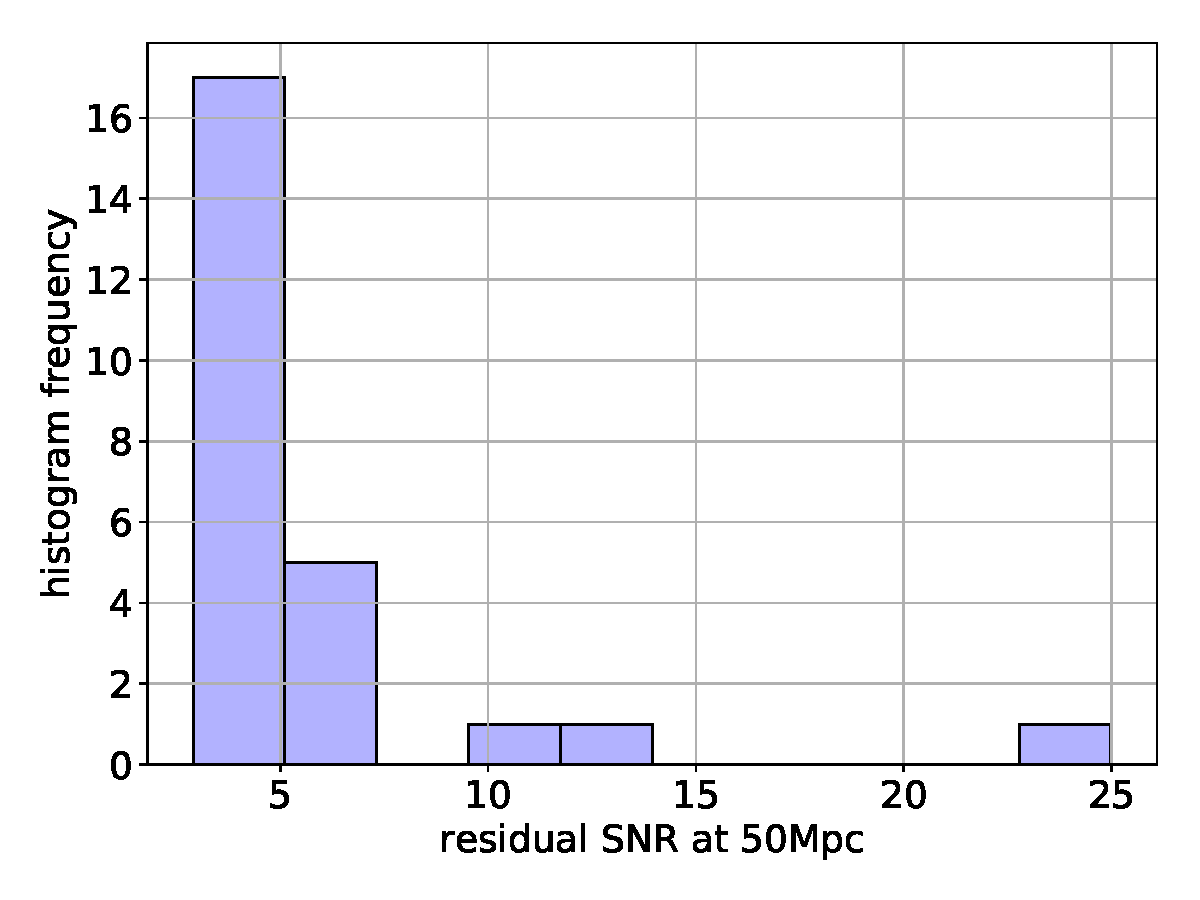
\includegraphics[width=10cm]{./img/CannonLogAmpPh-hist-cv.pdf} 
	\caption[\protect\input{./img/CannonLogAmpPh-Short-hist-cv.txt}]{\protect\input{./img/CannonLogAmpPh-hist-cv.txt}}
	\label{fig:CannonLogAmpPh-hist-cv}
\end{figure}
The residual SNR values range from around 2.0 to up to near 25, though the majority look to be less than 7.0. Furthermore, if waveforms with residual SNR above 7.0 are designated as outliers, then one of the test waveforms, ALF2/1.225M$_\odot$ falls into this category. Allowing for the removal of these outliers results in figure~\ref{fig:CannonLogAmpPh-noout-hist-cv}:
\begin{figure}[H]
	\centering
	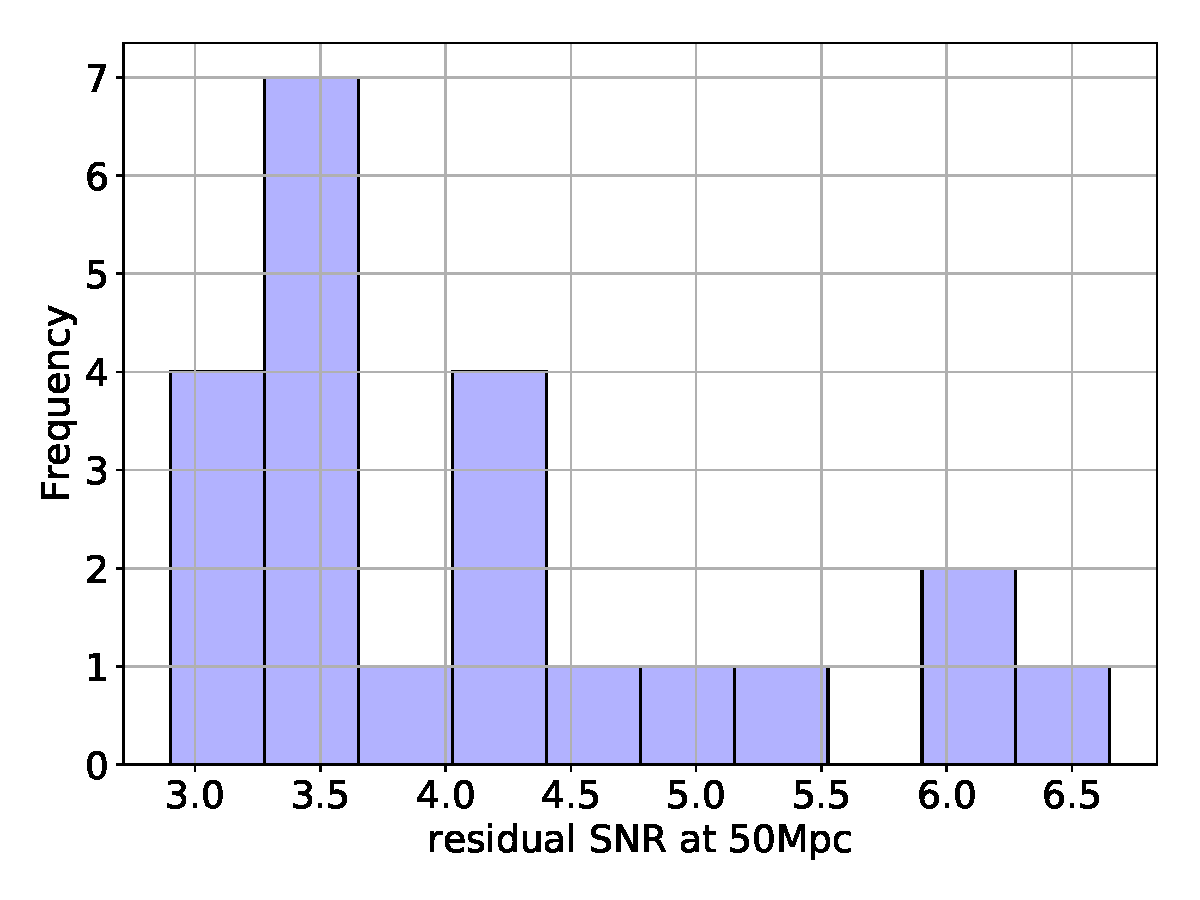
\includegraphics[width=10cm]{./img/CannonLogAmpPh-noout-hist-cv.pdf} 
	\caption[\protect\input{./img/CannonLogAmpPh-Short-noout-hist-cv.txt}]{\protect\input{./img/CannonLogAmpPh-noout-hist-cv.txt}}
	\label{fig:CannonLogAmpPh-noout-hist-cv}
\end{figure}
These residual SNR values still appear much too large even when the outliers have been removed and the machine learning algorithm should work with all waveforms, not just a selection of them. Therefore we do not wish to exclude any outliers. 

\subsubsection{Training on real and imaginary components of the Fourier transform of the signals}
It is possible that the large residual SNR values obtained in the previous section could be caused by the interaction between the learning algorithm and the wrapping of the phase. The SNR residual metric (see section~\ref{sec:SNRresidual}) compares the signals in the complex domain, so that a signal with a phase angle of slightly less than $\pi$ is similar to a signal with a phase angle of slightly larger than $-\pi$. Whereas The Cannon algorithm when supplied with phase information, considers these two signals widely apart. This could have been compensated for by adjusting the comparison metric, but time constraints prevented this modification of The Cannon 2 code. Wrapping the phase angle between $-\pi$ and $\pi$ did not help very much either. This is still likely to the learning algorithm not realising the proximity of $-\pi$ and $\pi$ as mentioned above. To investigate whether this was truly a factor in the poor performance of the system with complex values, the machine learning process was repeated while training on the real and imaginary parts of the Fourier spectra, rather than the amplitude and the phase of the spectra. \par
Figure~\ref{fig:CannonReImAPR4-q10-M1275} shows The Cannon response when trained on the real and imaginary parts of APR/1.275M$_\odot$: 
\begin{figure}[H]
	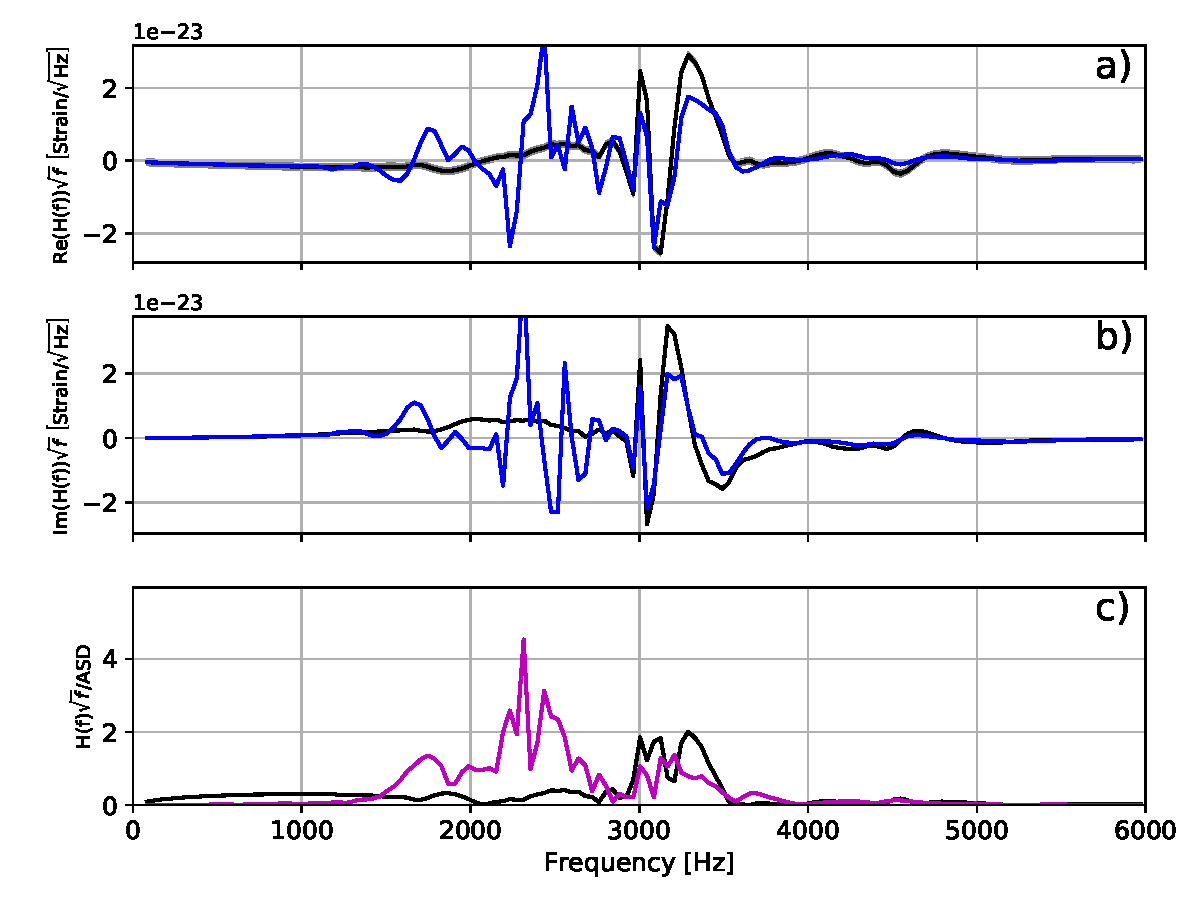
\includegraphics[width=15cm]{./img/CannonReImAPR4-q10-M1275.pdf} 
	\caption[\protect\input{./img/CannonReImAPR4-q10-M1275Short.txt}]{\protect\input{./img/CannonReImAPR4-q10-M1275.txt}}
	\label{fig:CannonReImAPR4-q10-M1275}
\end{figure}
The residual SNR has increased from 1.10 (figure~\ref{fig:CannonLogAmpPhAPR4-q10-M1275}) when trained on the amplitude and phase of the FFT, to 2.57 when trained on the corresponding real and imaginary parts. The visual correlation between the original image and the inferred image is quite poor which is reflected in the error function shown on part c) of the plot. The response for ALF2/1.225M$_\odot$ is shown in figure~\ref{fig:CannonReImALF2-q10-M1225}:
\begin{figure}[H]
	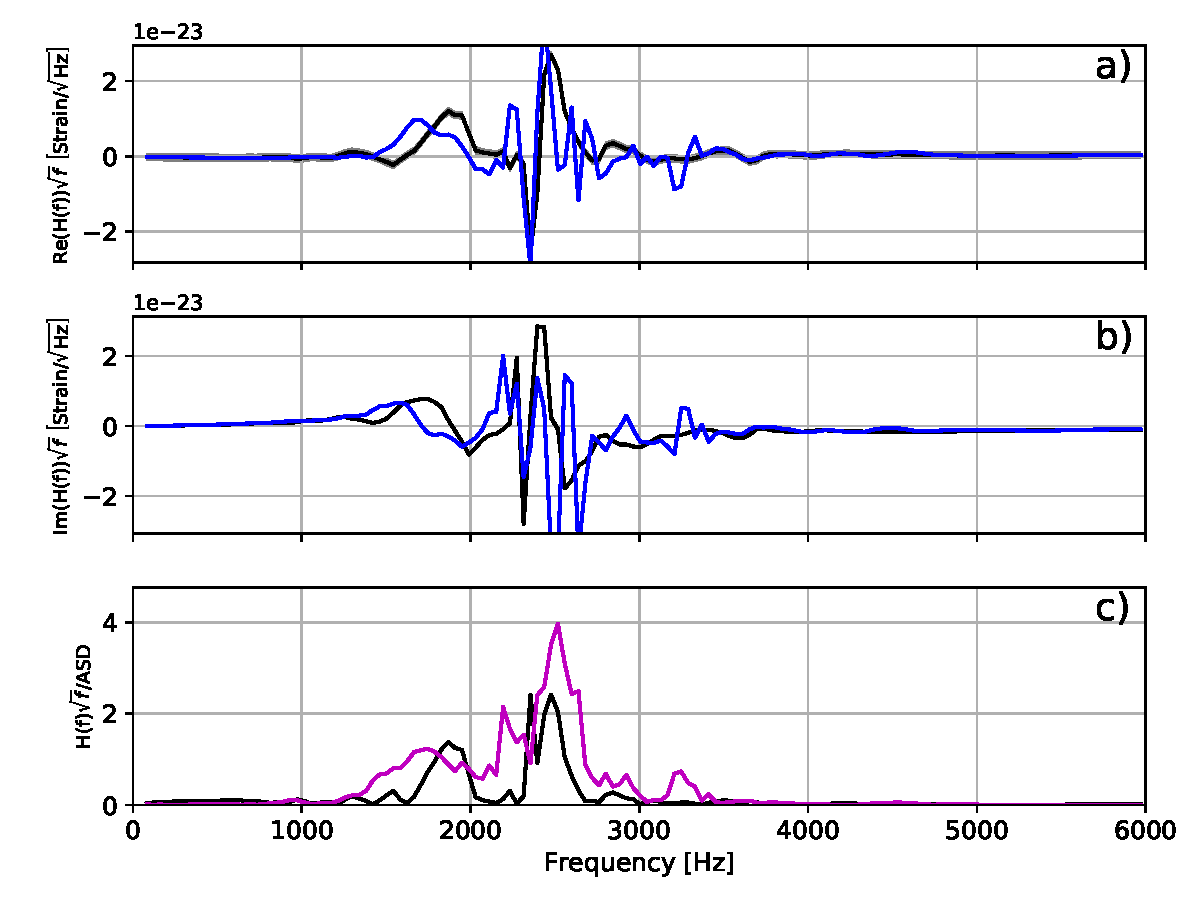
\includegraphics[width=15cm]{./img/CannonReImALF2-q10-M1225.pdf} 
	\caption[\protect\input{./img/CannonReImALF2-q10-M1225Short.txt}]{\protect\input{./img/CannonReImALF2-q10-M1225.txt}}
	\label{fig:CannonReImALF2-q10-M1225}
\end{figure}
Which coincidentally, also has a residual SNR of 2.57 with a previous residual SNR of 3.56 (figure~\ref{fig:CannonLogAmpPhALF2-q10-M1225}) which is a slight decrease. The performance of these two sample signals when learning on the real and imaginary parts of the FFT, without leave one out cross-validation, is  not significantly better than the those trained in the log amplitude phase phase. Furthermore, implementing leave one out cross-validation would deteriorate these results further. At this point in time we considered looking at another learning algorithm, random forest regression, which is examined in section~\ref{sec:RandomForest}.\\
\subsection{The Cannon 2 summary}
When we trained the Cannon 2 on the amplitude and phase information (see section~\ref{sec:TheCannonEntireTrainingSet}) we initially achieved reasonable results, however, this was when our waveform under test was included in the training set. Machine learning algorithms are routinely tested with "out of sample" data, in other words, the signal under test should be excluded from the training data. When we excluded our test waveform from the training set (section~\ref{sec:TheCannonLOOCV}) the residual SNR values increased dramatically to a range of values between 3 and 25 which is much too high for our application, where our goal is to achieve numbers much less than one for the residual SNR so that the reconstructed waveform is indistinguishable to the true waveform from the point of view of LIGO. We then altered our training method to train on the real and imaginary signals, to attempt to counteract any deterioration in performance due to phase errors. This did not result in any significant improvement. However, it must be noted that the training and prediction process for each waveform occur is a few seconds, so any future modifications that reduce the residual SNR are well worth implementing. 
\pagebreak
\subsection{Random forest analysis}
\label{sec:RandomForest}
For implementation of the random forest regression algorithm, we decided to implement a simplified frequency shift in both the real and imaginary components of the Fourier transform. Rather than use the more complex frequency multiplication, which required interpolation of the signals,  a frequency bin shifting algorithm was used (section~\ref{sec:PCAScaled}). Leave one out cross-validation was not performed in this section  as a method was required to calculate the frequency shift to reverse for a waveform excluded from training set, and this was a task set for future work.  The initial random seed was kept fixed in this section. 
\subsubsection{Inferred waveforms}
Figure~\ref{fig:RFRReImAPR4-q10-M1275} shows the waveform inferred from the random forest algorithm trained on the real and imaginary parts of the APR4/1.275M$_\odot$ with frequency bin shifting:
\begin{figure}[H]
	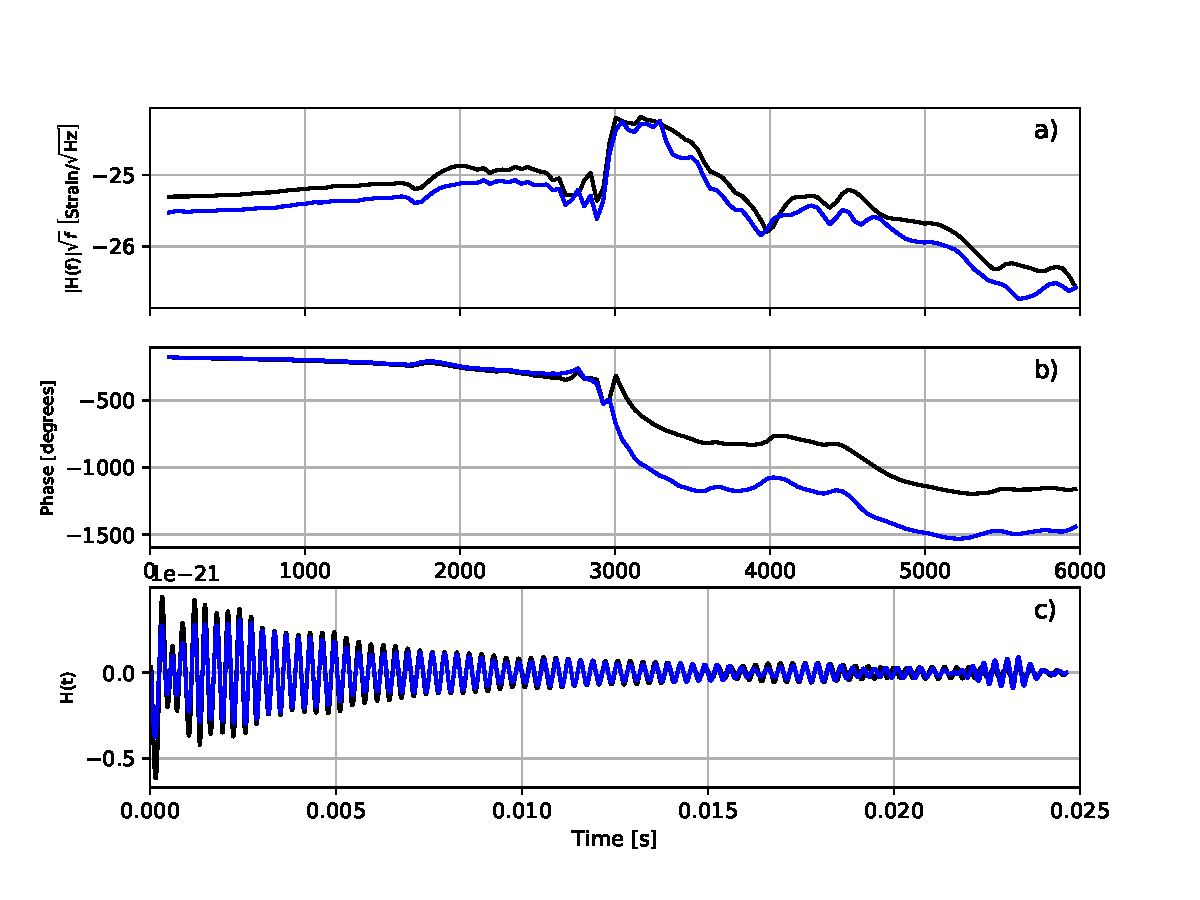
\includegraphics[width=15cm]{./img/RFRReImAPR4-q10-M1275.pdf} 
	\caption[\protect\input{./img/RFRReImAPR4-q10-M1275Short.txt}]{\protect\input{./img/RFRReImAPR4-q10-M1275.txt}}
	\label{fig:RFRReImAPR4-q10-M1275}
\end{figure}
The magnitude of the inferred signal in the frequency domain (blue curve plot a) is consistently lower than the original spectrum (black curve plot a), resulting in a time domain signal that underestimates the original signal. The zero crossing in the time domain of the inferred waveform and original signal align well up to 18ms and loose synchronisation after this time. The inferred signal has a residual SNR of 0.71 which is reasonably low, but this does not include cross-validation. Looking now at the other signal, the random forest response to ALF2/1.225M$_\odot$ is shown in figure~\ref{fig:RFRReImALF2-q10-M1225}:
\begin{figure}[H]
	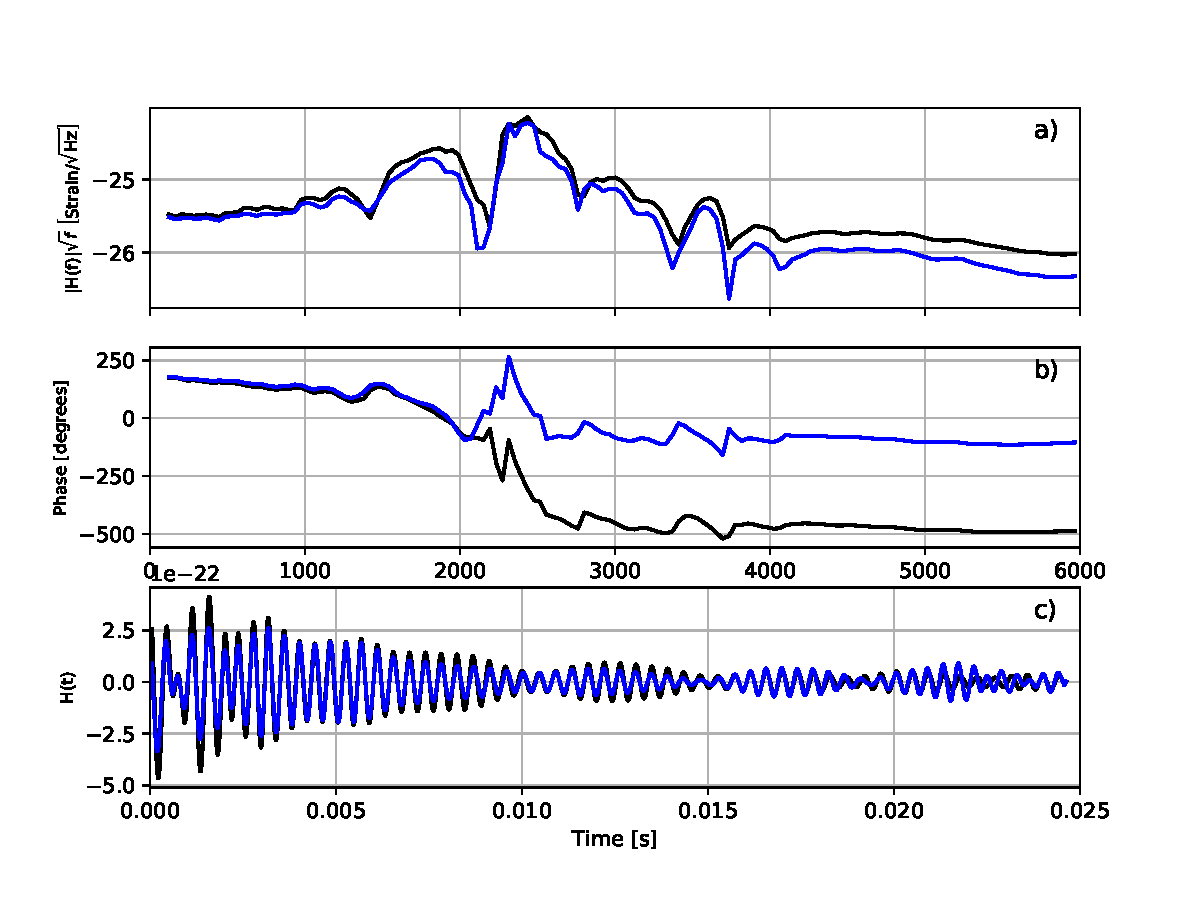
\includegraphics[width=15cm]{./img/RFRReImALF2-q10-M1225.pdf} 
	\caption[\protect\input{./img/RFRReImALF2-q10-M1225Short.txt}]{\protect\input{./img/RFRReImALF2-q10-M1225.txt}}
	\label{fig:RFRReImALF2-q10-M1225}
\end{figure}
As with figure~\ref{fig:RFRReImAPR4-q10-M1275}, the synchronisation in the time domain aligns well for time periods less than 18ms, but the amplitude of the time domain signal is consistently underestimated, particularly immediately after merger when the signal strength is largest. The residual SNR for this waveform is 0.80, slightly larger than APR4/1.276M$_\odot$. Now that the sample signals have been analysed, the residual SNR values can be determined for all the signals, this was calculated and shown in the  histogram in figure~\ref{fig:RFRReImHist}:
\begin{figure}[H]
	\centering
	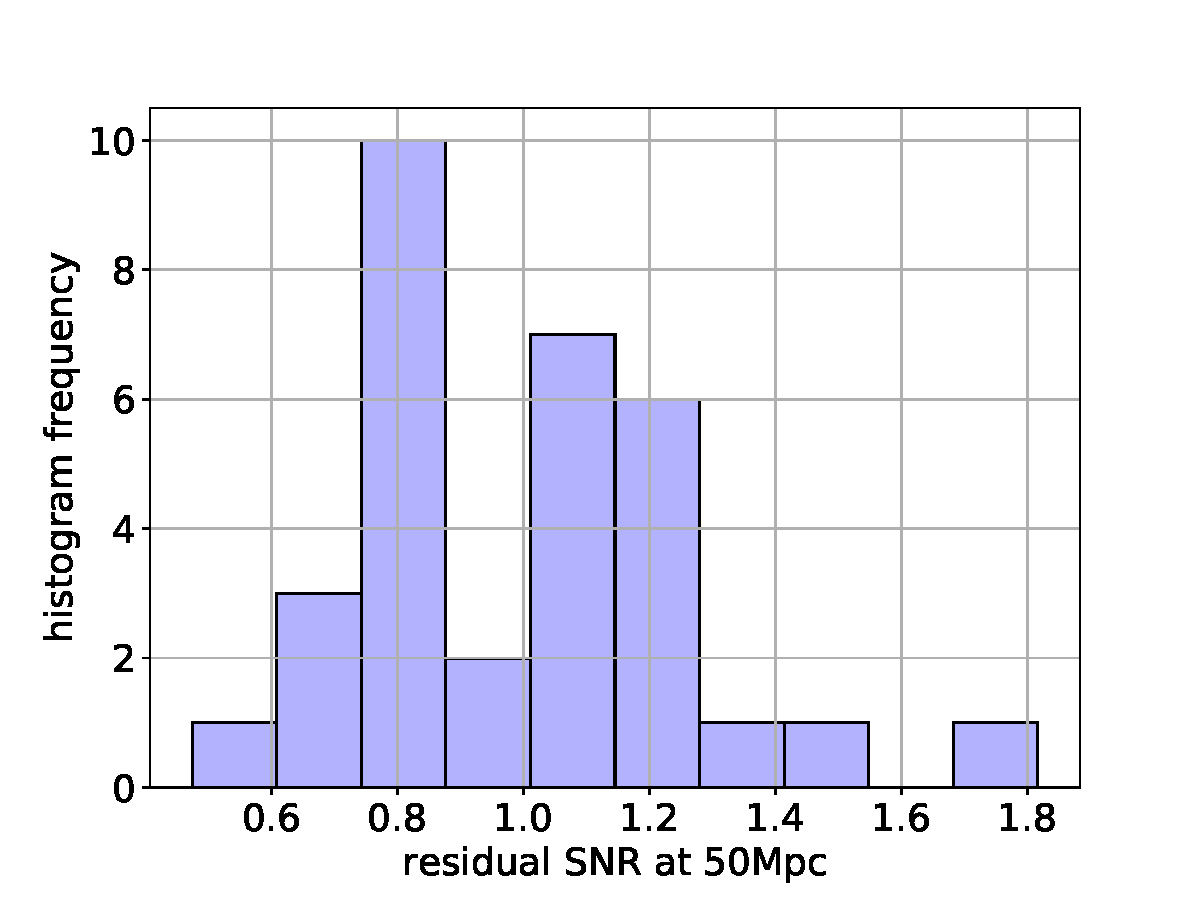
\includegraphics[width=10cm]{./img/RFRReImHist.pdf} 
	\caption[\protect\input{./img/RFRReImHistShort.txt}]{\protect\input{./img/RFRReImHist.txt}}
	\label{fig:RFRReImHist}
\end{figure}
The residual SNR is less than 1.8 for all waveforms, though this was achieved without cross-validation. These values are still too high for our purposes as residual SNR values of less than 1.0 are required, and it should also be noted that a stronger signal will result in a larger residual SNR. Figure~\ref{fig:RFRReImHist} has been generated from the random forest algorithm with a fixed random seed, the next figures investigate the effect of the random seed on the residual SNR values. Figure~\ref{fig:RFRRandomseed} shows the mean residual SNR when run with 100 different random seeds:
\begin{figure}[H]
	\centering
	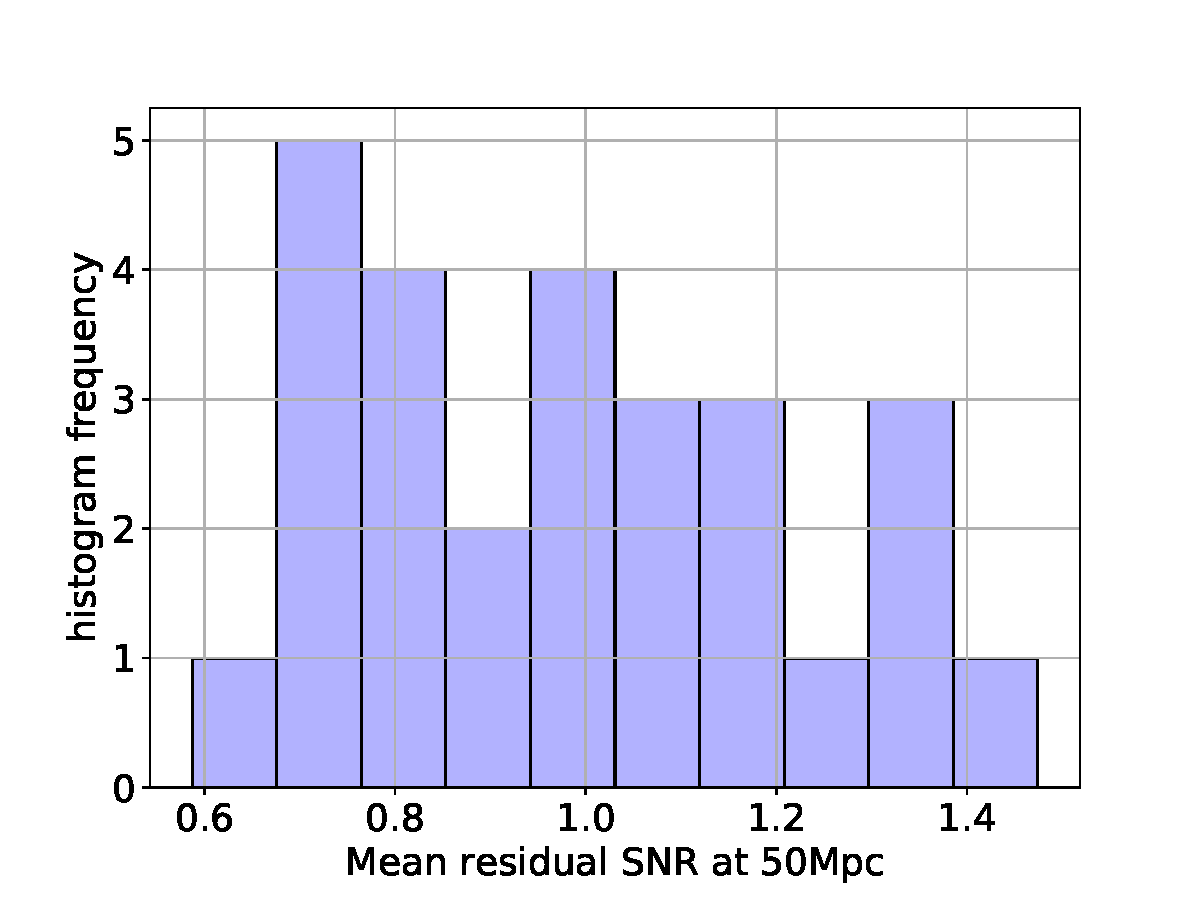
\includegraphics[width=10cm]{./img/RFRRandomseed.pdf} 
	\caption[\protect\input{./img/RFRRandomseedShort.txt}]{\protect\input{./img/RFRRandomseed.txt}}
	\label{fig:RFRRandomseed}
\end{figure}
The upper limit of the mean residual SNR is slightly less than the value obtained in figure~\ref{fig:RFRReImHist}, but otherwise the range of values is essentially the same, from 0.6 to 1.5, indicating that the random forest algorithm is relatively independent of the initial random seed chosen. This can be explored further by visualising the relationship of the random seeds on individual EOS/mass combinations as shown in figure~\ref{fig:RFRresidualBoxEOSsorted}: 
\begin{figure}[H]
	\centering
	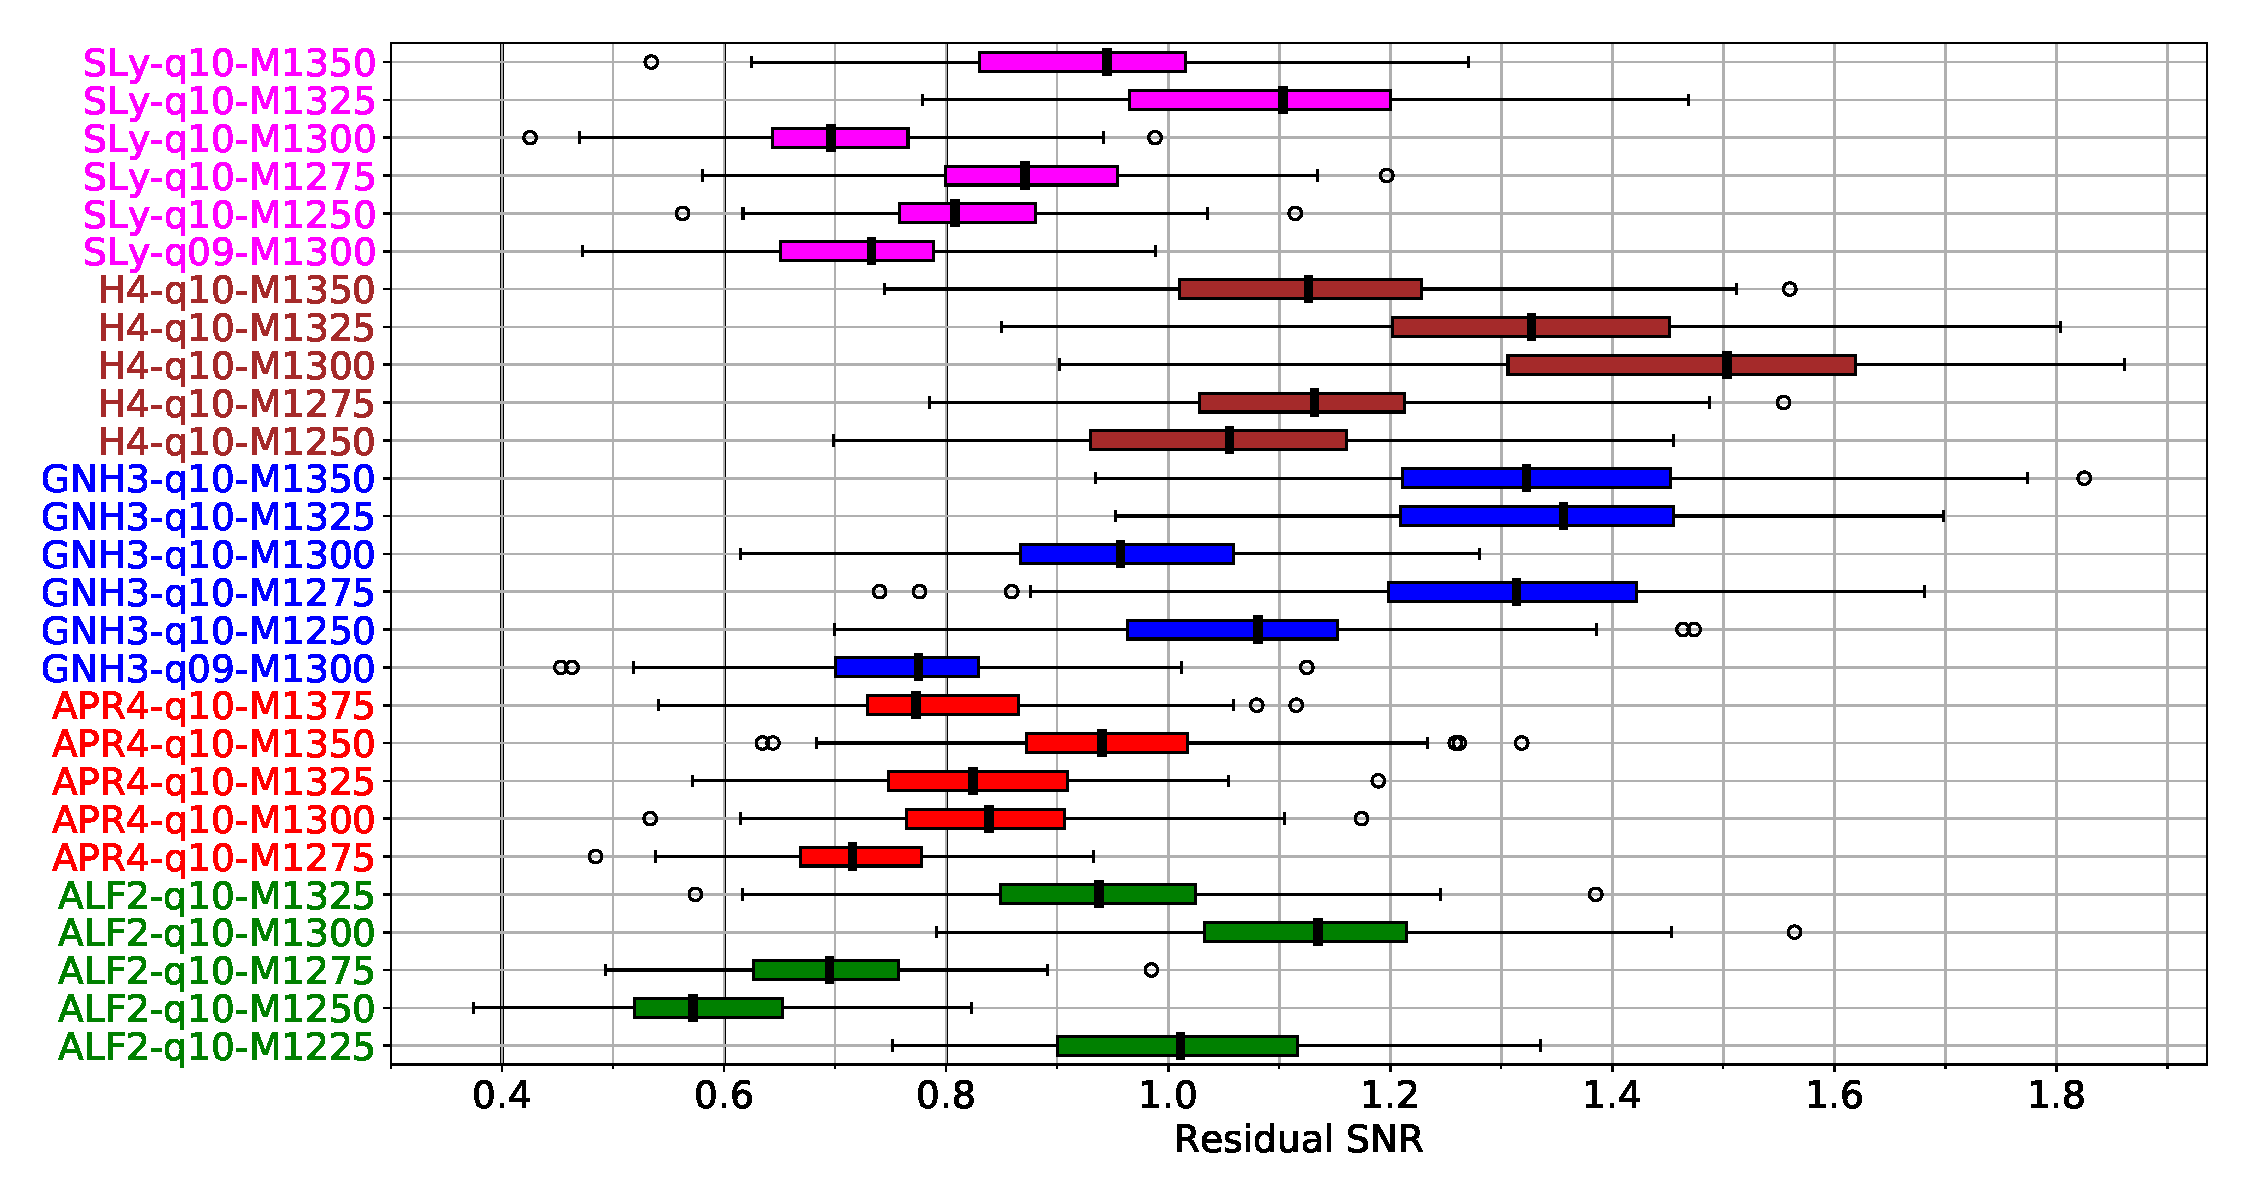
\includegraphics[width=15cm]{./img/RFRresidualBoxEOSsorted.pdf} 
	\caption[\protect\input{./img/RFRresidualBoxEOSsortedShort.txt}]{\protect\input{./img/RFRresidualBoxEOSsorted.txt}}
	\label{fig:RFRresidualBoxEOSsorted}
\end{figure}
The box plot has been sorted by EOS and mass and coloured the same way as in figures~\ref{fig:hEOS}~and~\ref{fig:fEOS}. The residual SNR scores appear to be consistently distributed for each input waveform combination, though outliers (circles) do tend to appear occasionally. The variation of the residual SNR over the interquartile range is around $\pm$0.1 to $\pm$0.2, whereas the variation over the minumum and maximum values, excluding outliers, varies up to $\pm$0.5. If these waveforms were generated with cross-validation, it would be expected that the lowest and the largest mass values, for a given EOS would have a larger residual SNR due to the position on the extrema of the waveforms, though this is not generally the case here. It is also instructive to sort these values by the mean residual SNR and this is shown in figure~\ref{fig:RFRresidualBoxEOSsorted}:
\begin{figure}[H]
	\centering
	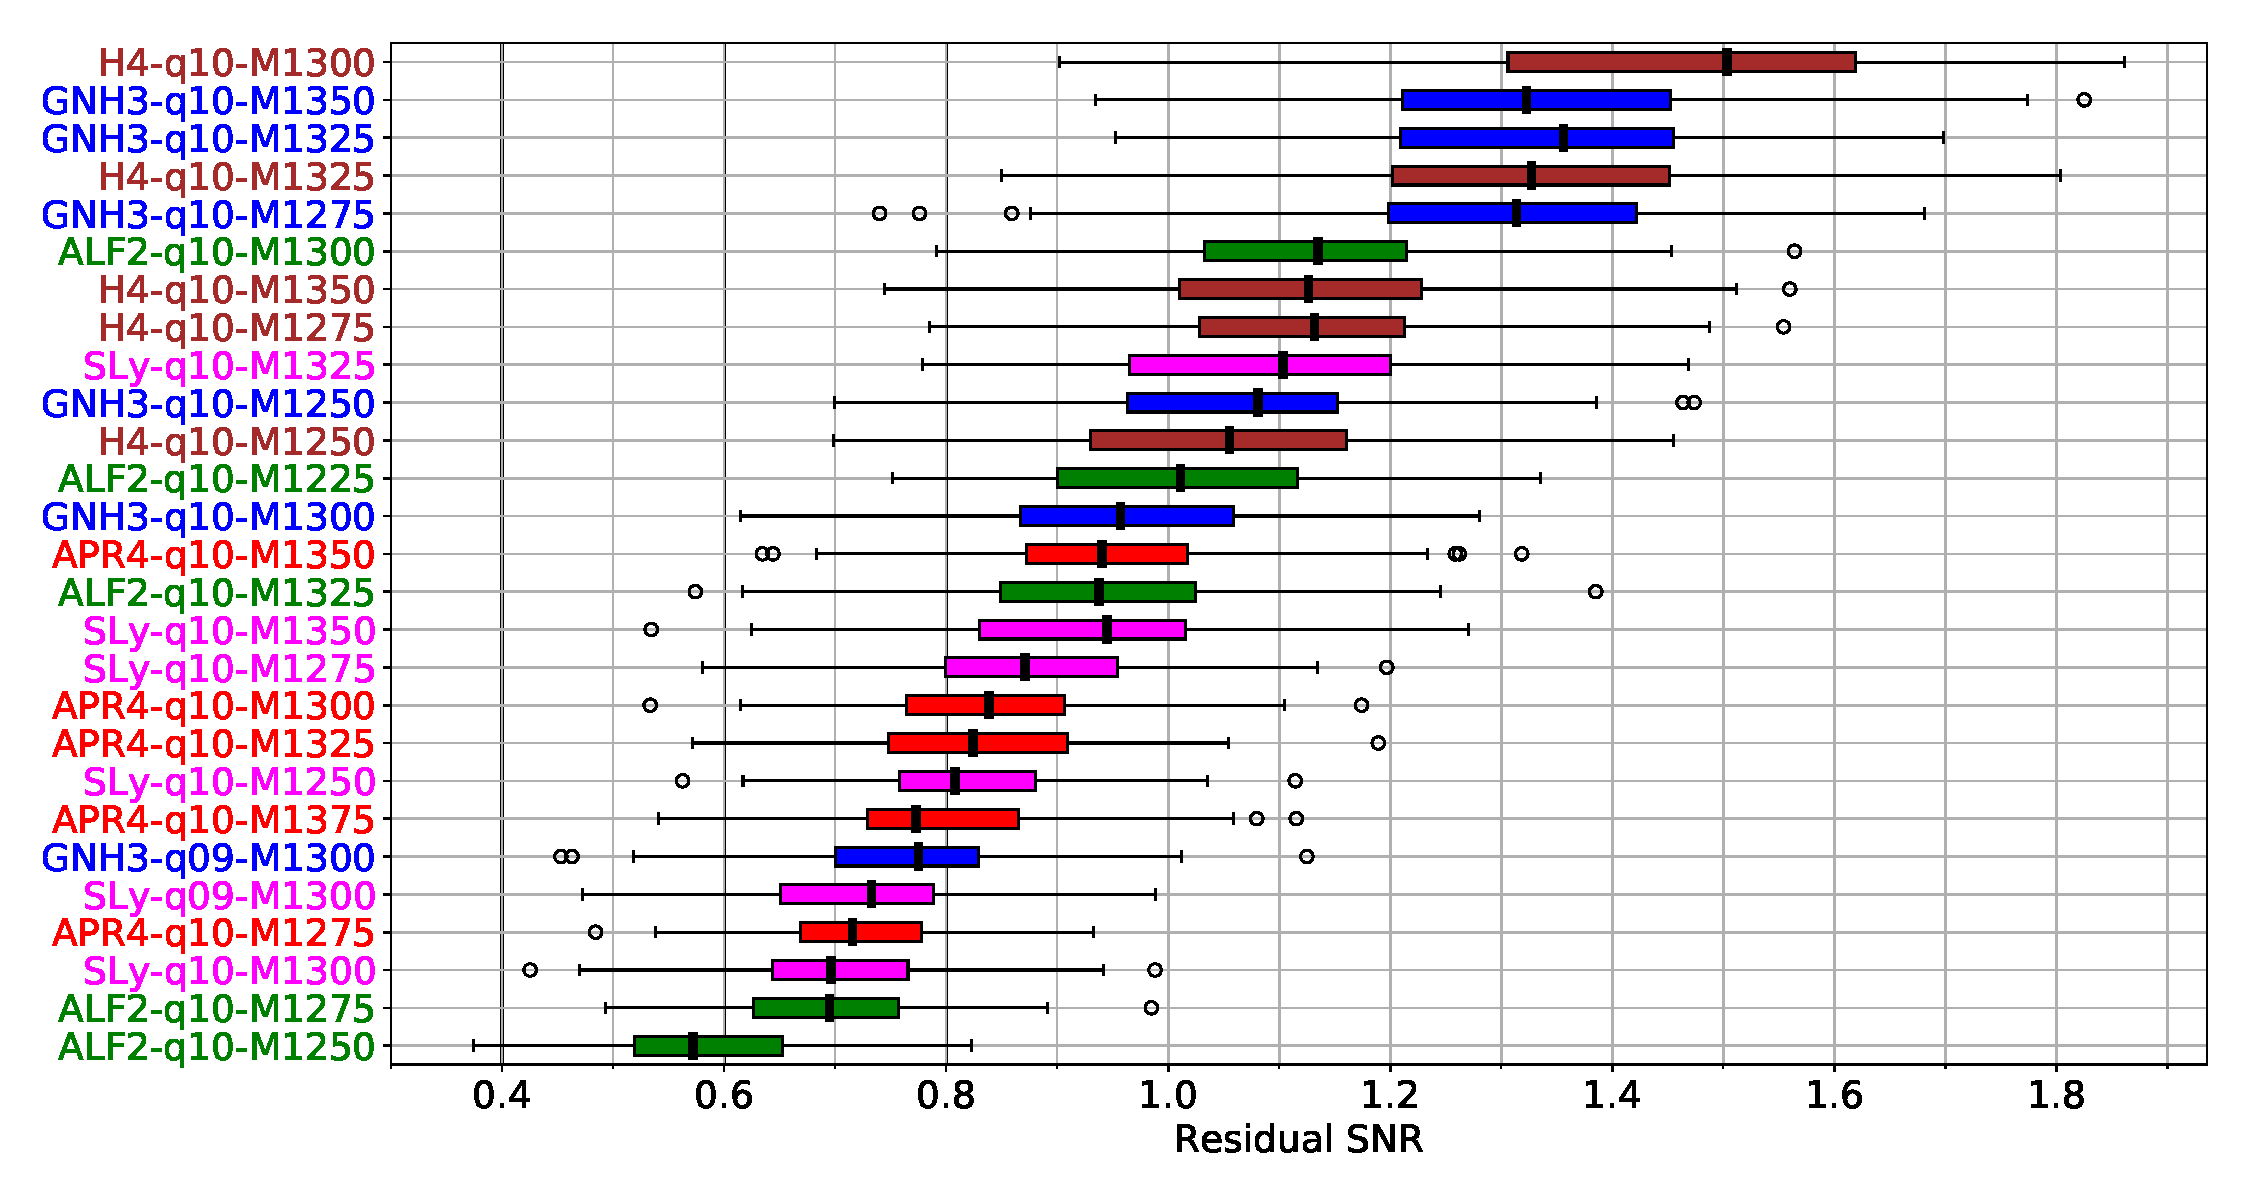
\includegraphics[width=15cm]{./img/RFRresidualBoxMeansorted.pdf} 
	\caption[\protect\input{./img/RFRresidualBoxMeansortedShort.txt}]{\protect\input{./img/RFRresidualBoxMeansorted.txt}}
	\label{fig:RFRresidualBoxMeansorted}
\end{figure}
This box plot shows the waveforms ranked by residual SNR for the random forest algorithm. This shows that ALF2/1.250M$_\odot$ is consistently the best match of all the waveforms, and that H4/1.300M$_\odot$ is consistently the worse match of all the waveforms. Comparison of figure~\ref{fig:RFRresidualBoxMeansorted} to the scaled PCA decomposition is figures~\ref{fig:PCAScaled3Damp}-\ref{fig:PCAScaled2Dphase} yields no obvious connection other than the worst four waveforms (H4-q10-M1325 to H4-q10-M1300 on this plot) tend to be outliers on the amplitude of the PCA space, but that is quite a weak relationship. This plot also shows where the test waveforms fall in terms of the other waveforms. APR-q10-M1275 has the fourth lowest residual SNR with  a value of around 0.7, and ALF2-q10-M1225 is mid-ranged with a value of around 1.0. Both these values are consistent with previous results.\par 

One particularly useful parameter available to random forest decision trees is the ability to ascertain which inputs were most important in determining the output waveforms. This parameter is known as the relative importance and is shown in figure~\ref{fig:RFRelativeLabelImportance}. 
\begin{figure}[H]
		\centering
		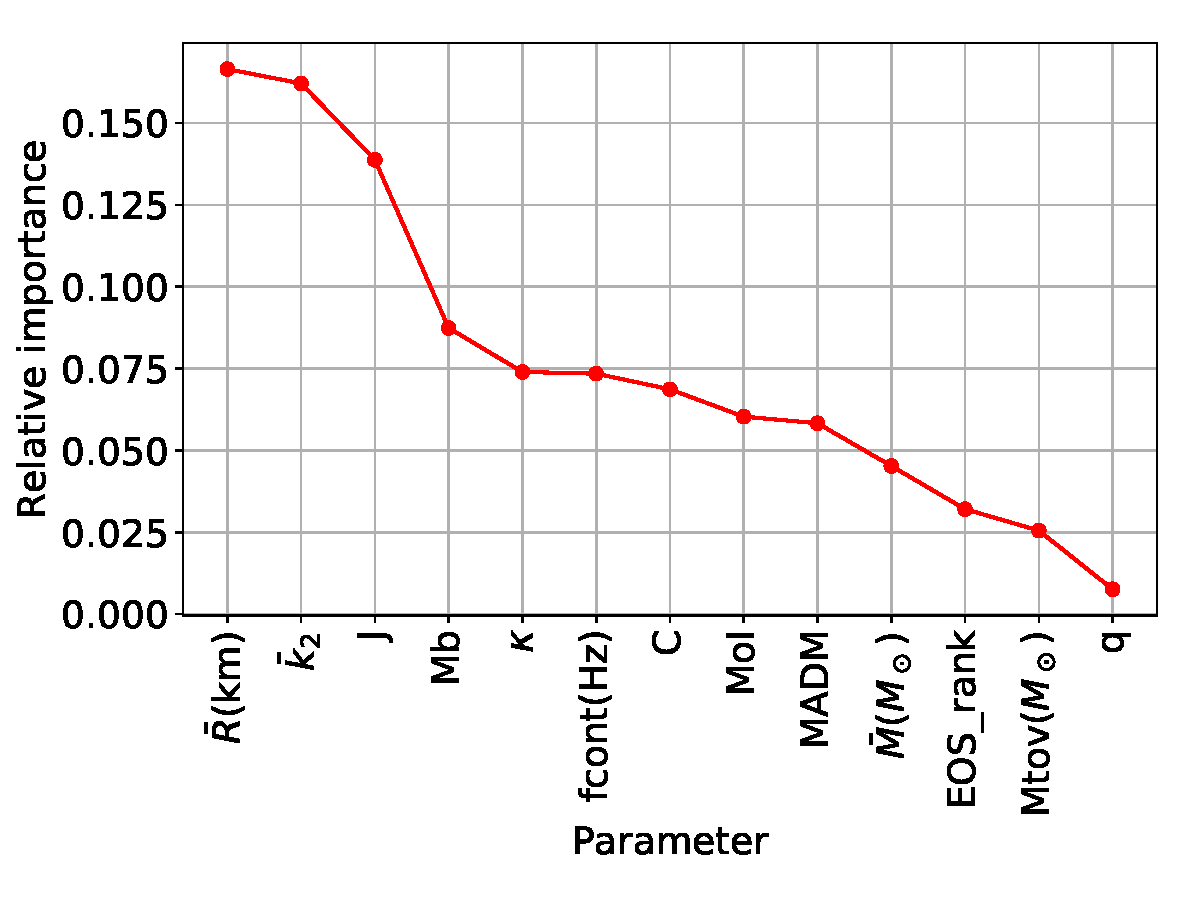
\includegraphics[height=8.0cm]{./img/RFRelativeLabelImportance.pdf} 
		\caption[\protect\input{./img/RFRelativeLabelImportanceShort.txt}]{\protect\input{./img/RFRelativeLabelImportance.txt}}
		\label{fig:RFRelativeLabelImportance}
\end{figure}
Out of the thirteen input parameters for each waveform, 47\% of the decisions made for signal generation was made with from the mean neutron star radius, $\bar{\text{R}}$, the Love 2 tidal parameter $\bar{k}_2$ and the initial angular momentum of the system $J$. It also is interesting to note from figure~\ref{fig:RFRelativeLabelImportance} that the neither of the three most important properties of the reconstruction include the EOS, or mass values. Nevertheless, the EOS properties are implicitly encoded in the mean neutron star radius and the tidal Love number, and the mass values are encoded in the initial angular momentum of the system.
\subsubsection{Random forest summary}
The random forest algorithm generated waveforms with lower residual SNR than The Cannon 2, however, at this point in time, cross-validation was not implemented in the random forest algorithm. Without cross-validation, the random forest regressor was able to create waveforms that were getting close to the required accuracy, with residual SNR values in the range of 0.6 to 1.5, but these values are still too large. The goal for the residual SNR value is less than one and this is dependent on the initial signal strength. The waveforms used in this thesis were normalised to a BNS event at 50Mpc, if the event occurred further out then a smaller residual SNR would be observed. The random forest algorithm was consistent due to variations in the initial random number seed, however, outliers were observed with maximum values for residual SNR that can exceed 1.8. The ratio of the residual SNR to signal SNR varied from 0.22 to 0.62, if the incoming signal SNR had a detectable value of 5.0 to allow detection, then to obtain a residual SNR of less than 1.0 requires that the ratio is less than 0.2 which is below the lower limit. These problems could possibly be related to the lack of test waveforms which leaves open the following question "How many waveforms do we need to get acceptable residual SNR" and this is a question for future work. 



% RF_SNR_Comp.ods

\section{Future tasks}
This project was performed with 25 numerical waveforms, this is a small amount for machine learning. It is possible that a significant improvement may occur in the predictions of The Cannon 2, and random forest, if more numerical relativity waveforms were used. The random forest algorithm could be modified to learn the frequency shift amount so that a full leave one out cross-validation process can be performed. 

